% ***************************************************************************************************
%
%	Szablon pracy magisterskiej dla Politechniki Wrocławskiej w wersji dwustronnej.
%	Autor:	Tomasz Strzałka
%
% ***************************************************************************************************

% Styl dwustronny z domyślną wielkością czcionki 10pt oraz oddzieloną stroną tytułową (titlepage).
% Domyślnie rodziały rozpoczynają się na stronie prawej (openright).
\documentclass{book}

% ***************************************************************************************************
% Ustawienia języka
% ***************************************************************************************************

% Podstawowe ustawienia języka, według którego formatowany będzie dokument
\usepackage[english]{babel}
\usepackage{csquotes}
% Pakiet babel dla polskiego języka powoduje konflikt z pakietem amssymb.
% Polecenie '\lll' definiują oba pakiety - porządana jest druga definicja.

% W przypadku wielojęzykowości ustawia główny język dokumentu
\selectlanguage{english}

% Kodowanie dokumentu
\usepackage[utf8]{inputenc}

% Dowolny rozmiar czcionek, kodowanie znaków
\usepackage{lmodern}

% Polskie wcięcia akapitów
% \usepackage{indentfirst}

% Polskie łamanie wyrazów
% \usepackage[plmath]{english}

% Przecinek w wyrażeniach matematycznych zamiast kropki
% \usepackage{icomma}

% Polskie formatowanie typograficzne
% \frenchspacing

% Zapewnia liczne usprawnienia wyświetlania i organizacji matematycznych formuł. 
\usepackage{amsmath}

% Wprowadza rozszerzony zestaw symboli m.in. \leadsto
\usepackage{amssymb}

% Dodatkowa, ,,kręcona'' czcionka matematyczna
\usepackage{mathrsfs}

% Dodatkowe wsparcie dla środowiska mathbb, które nie wspiera domyślnie cyfr (\mathbb{})
\usepackage{bbold}

% Fixes/improves amsmath
\usepackage{mathtools}



% ***************************************************************************************************
% Kolory  
% ***************************************************************************************************

% Umożliwia kolorowanie poszczególnych komórek tabeli
\usepackage[table]{xcolor}% http://ctan.org/pkg/

% Umożliwia łatwą zmianę koloru linii w tabeli
\usepackage{tabu}

% Umożliwia rozszerzoną kontrolę nad kolorami.
\usepackage{xcolor}

% Definicje kolorów
\definecolor{lgray}{HTML}{9F9F9F}
\definecolor{dgray}{HTML}{5F5F5F}
% lgray				-	nazwa nowo zdefiniowanego koloru
% HTML				-	model kolorów
% CCCCCC			-	wartość koloru zgodna z modelem

% ***************************************************************************************************
% Algorytmy 
% ***************************************************************************************************

% Udostępnia środowisko do konstruowania pseudokodów
% \usepackage[ruled,vlined,linesnumbered,longend,algochapter]{algorithm2e}
% ruled	- poziome kreski na początku i końcu algorytmu, podpis na górze oddzielony również kreską poziomą
% vlined - pionowe kreski łączące początek polecenia z jego końcem
% linesnumbered	- numerowanie kolejnych wierszy algorytmu
% longend - długie końcówki np. ifend, forend itd.
% algochapter - numeracja z rozdziałami

% Zmiana rozmiaru komentarzy
% \newcommand\algcomment[1]{
	% \footnotesize{#1}
% }

% Ustawienie zadanego stylu dla komentarzy
% \SetCommentSty{algcomment}

% Wyśrodkowana tylda
\usepackage{textcomp}%
\newcommand{\textapprox}{\raisebox{0.5ex}{\texttildelow}}

% Listowanie kodów źródłowych
\usepackage{listings} 

% ***************************************************************************************************
% Marginesy 
% ***************************************************************************************************

% Ustawienia rozmiarów stron i ich marginesów
\usepackage[headheight=18pt, top=25mm, bottom=25mm, left=25mm, right=25mm]{geometry}
% headheight		-	wysokość tytułów
% top				-	margines górny
% bottom			-	margines dolny
% left				-	margines lewy
% right				-	margines prawy

% Usunięcie górnego marginesu dla środowisk
\makeatletter
\setlength\@fptop{0\p@}	
\makeatother

% ***************************************************************************************************
% Styl 
% ***************************************************************************************************

% Definiuje środowisko 'titlingpage', które zapewnia pełną kontrolę nad układem strony tytułowej.
\usepackage{titling}


% Umożliwia modyfikowanie stylu spisu treści
\usepackage{tocloft}	

\tocloftpagestyle{tableOfContentStyle}

% Definiowanie własnych stylów nagłówków i/lub stopek
\usepackage{fancyhdr}

% Domyślny styl dla pracy 
\fancypagestyle{custom}{
	\fancyhf{}									% wyczyść stopki i nagłówki
	\fancyhead[RO]{								% Prawy, nieparzysty nagłówek
		\hrulefill \hspace{16pt} \large Chapter \thechapter
		\put(-472.1, 13.5){%
			\makebox(0,0)[l]{%
				
\includegraphics[width=0.05\textwidth]{Figures/pwr-logo}
			}
		}
		\put(-443,5.5){%
			\makebox(0,0)[l]{%
				\small Wrocław University of Science and Technology
			}
		}
	}
	\fancyhead[LE]{								% Lewy, parzysty nagłówek
		\large Chapter \thechapter \hspace{16pt} \hrulefill 
		\put(-22, 12.1){%
			\makebox(0,0)[l]{%
				
\includegraphics[width=0.05\textwidth]{Figures/wppt-logo}
			}
		}
		\put(-220,5.5){%
			\makebox(0,0)[l]{%
				\small Faculty of Fundamental Problems of Technology
			}
		}
	}
	\fancyfoot[LE,RO]{							% Stopki
		\thepage
	}
	\renewcommand{\headrulewidth}{0pt}			% Grubość linii w nagłówku
	\renewcommand{\footrulewidth}{0.2pt}		% Grubość linii w stopce
}


% Domyślny styl dla bibliografii
\fancypagestyle{bibliographyStyle}{
	\fancyhf{}									% wyczyść stopki i nagłówki
	\fancyhead[RO]{								% Prawy, nieparzysty nagłówek
		\hrulefill \hspace{16pt} \large Appendix \thechapter
		\put(-472.1, 13.5){%
			\makebox(0,0)[l]{%
				
\includegraphics[width=0.05\textwidth]{Figures/pwr-logo}
			}
		}
		\put(-443,5.5){%
			\makebox(0,0)[l]{%
				\small Wrocław University of Science and Technology
			}
		}
	}
	\fancyhead[LE]{								% Lewy, parzysty nagłówek
		\large Bibliography \hspace{16pt} \hrulefill 
		\put(-22, 12.1){%
			\makebox(0,0)[l]{%
				
\includegraphics[width=0.05\textwidth]{Figures/wppt-logo}
			}
		}
		\put(-220,5.5){%
			\makebox(0,0)[l]{%
				\small Faculty of Fundamental Problems of Technology
			}
		}
	}
	\fancyfoot[LE,RO]{							% Stopki
		\thepage
	}
	\renewcommand{\headrulewidth}{0pt}			% Grubość linii w nagłówku
	\renewcommand{\footrulewidth}{0.2pt}		% Grubość linii w stopce
}

% Domyślny styl dla dodatków
\fancypagestyle{appendixStyle}{
	\fancyhf{}									% wyczyść stopki i nagłówki
	\fancyhead[RO]{								% Prawy, nieparzysty nagłówek
		\hrulefill \hspace{16pt} \large Appendix \thechapter
		\put(-472.1, 13.5){%
			\makebox(0,0)[l]{%
				
\includegraphics[width=0.05\textwidth]{Figures/pwr-logo}
			}
		}
		\put(-443,5.5){%
			\makebox(0,0)[l]{%
				\small Wrocław University of Science and Technology
			}
		}
	}
	\fancyhead[LE]{								% Lewy, parzysty nagłówek
		\large Appendix \thechapter \hspace{16pt} \hrulefill 
		\put(-22, 12.1){%
			\makebox(0,0)[l]{%
				
\includegraphics[width=0.05\textwidth]{Figures/wppt-logo}
			}
		}
		\put(-210,5.5){%
			\makebox(0,0)[l]{%
				\small Faculty of Fundamental Problems of Technology
			}
		}
	}
	\fancyfoot[LE,RO]{							% Stopki
		\thepage
	}
	\renewcommand{\headrulewidth}{0pt}			% Grubość linii w nagłówku
	\renewcommand{\footrulewidth}{0.2pt}		% Grubość linii w stopce
}

% Osobny styl dla stron zaczynających rozdział/spis treści itd. (domyślnie formatowane jako "plain")
\fancypagestyle{chapterBeginStyle}{
	\fancyhf{}%
	\fancyfoot[LE,RO]{
		\thepage
	}
	\renewcommand{\headrulewidth}{0pt}
	\renewcommand{\footrulewidth}{0.2pt}
}

% Styl dla pozostałych stron spisu treści
\fancypagestyle{tableOfContentStyle}{
	\fancyhf{}%
	\fancyfoot[LE,RO]{
		\thepage
	}
	\renewcommand{\headrulewidth}{0pt}
	\renewcommand{\footrulewidth}{0.2pt}
}

% Formatowanie tytułów rozdziałów i/lub sekcji
\usepackage{titlesec}

% Formatowanie tytułów rozdziałów
\titleformat{\chapter}[hang]					% kształt
{
	\vspace{-10ex}
	\Huge
	\bfseries
}												% formatowanie tekstu modyfikowanego elementu
{}												% etykieta występująca przed tekstem modyfikowanego elementu, niewidoczna w spisie treści
{
	10pt
}												% odstęp formatowanego tytułu od lewego marginesu/etykiety
{
	\Huge
	\bfseries
}												% formatowanie elementów przed modyfikowanym tytułem
[
\vspace{2ex}
%\rule{\textwidth}{0.4pt}
%\vspace{-4ex}
]												% dodatkowe formatowanie stosowane poniżej modyfikowanego tytułu


% Formatowanie tytułów sekcji
\titleformat{\section}[hang]					% kształt
{
	\vspace{2ex}
%	\titlerule\vspace{1ex}
	\Large\bfseries
}												% formatowanie tekstu modyfikowanego elementu
{
	\thesection									% etykieta występująca przed tekstem modyfikowanego elementu, niewidoczna w spisie treści
}
{
	0pt
}												% odstęp formatowanego tytułu od lewego marginesu/etykiety
{
	\Large
	\bfseries
}												% formatowanie elementów przed modyfikowanym tytułem

% ***************************************************************************************************
% Linki
% ***************************************************************************************************

% Umożliwia wstawianie hiperłączy do dokumentu
\usepackage{hyperref}							% Aktywuje linki

\hypersetup{
	colorlinks	=	true,					% Koloruje tekst zamiast tworzyć ramki.
	linkcolor		=	blue,					% Kolory: referencji,
        citecolor		=	blue,					% cytowań,
	urlcolor		=	blue					% hiperlinków.
}

% Do stworzenia hiperłączy zostanie użyta ta sama (same) czcionka co dla reszty dokumentu
\urlstyle{same}




% ***************************************************************************************************
% Linki
% ***************************************************************************************************

% Umożliwia zdefiniowanie własnego stylu wyliczeniowego
\usepackage{enumitem}

% Nowa lista numerowana z trzema poziomami
\newlist{myitemize}{itemize}{3}

% Definicja wyglądu znacznika pierwszego poziomu
\setlist[myitemize,1]{
	label		=	\textbullet,
	leftmargin	=	4mm}

% Definicja wyglądu znacznika drugiego poziomu
\setlist[myitemize,2]{
	label		=	$\diamond$,
	leftmargin	=	8mm}

% Definicja wyglądu znacznika trzeciego poziomu
\setlist[myitemize,3]{
	label		=	$\diamond$,
	leftmargin	=	12mm
}


% ****************************** Biblatex ***********************************************************
\usepackage[
    backend=biber,
    style=numeric,
	sorting=none
  ]{biblatex}
\addbibresource{qliom.bib}

% ***************************************************************************************************


% ***************************************************************************************************
% Inne pakiety
% ***************************************************************************************************

% Dołączanie rysunków
\usepackage{graphicx}

% Figury i przypisy
\usepackage{caption}
\usepackage{subcaption}

% Umożliwia tworzenie przypisów wewnątrz środowisk
\usepackage{footnote}

% Umożliwia tworzenie struktur katalogów
\usepackage{dirtree}

% Rozciąganie komórek tabeli na wiele wierszy
\usepackage{multirow}

% Precyzyjne obliczenia szerokości/wysokości dowolnego fragmentu wygenerowanego przez LaTeX
\usepackage{calc}

% my packages
\usepackage{physics}
\usepackage{microtype}
\usepackage{cancel}
\usepackage{color}
\renewcommand{\CancelColor}{\color{red}}
\usepackage{lipsum}

\usepackage{epigraph}
\setlength\epigraphwidth{16cm}
\setlength\epigraphrule{0pt}

\usepackage{etoolbox}
\makeatletter
\patchcmd{\epigraph}{\@epitext{#1}}{\itshape\@epitext{#1}}{}{}
\makeatother

\usepackage{tikz}
\usetikzlibrary{shapes,arrows,decorations.pathreplacing}

% ***************************************************************************************************
% Matematyczne skróty
% ***************************************************************************************************

% Skrócony symbol liczb rzeczywistych
\newcommand{\RR}{\mathbb{R}}

% Skrócony symbol liczb naturalnych
\newcommand{\NN}{\mathbb{N}}

% Skrócony symbol liczb wymiernych
\newcommand{\QQ}{\mathbb{Q}}

% Skrócony symbol liczb całkowitych
\newcommand{\ZZ}{\mathbb{Z}}

% Skrócony symbol logicznej implikacji
\newcommand{\IMP}{\rightarrow}

% Skrócony symbol  logicznej równoważności
\newcommand{\IFF}{\leftrightarrow}

% Symbole operatorów spinowych
\newcommand{\Id}{\mathcal{I}}
\newcommand{\Sp}{S^{+}}
\newcommand{\Sm}{S^{-}}
\newcommand{\Sz}{S^{z}}
\newcommand{\Sx}{S^{x}}
\newcommand{\Sy}{S^{y}}
\newcommand{\hs}[2]{\left(#1 \middle| #2\right)}

% ***************************************************************************************************
% Środowiska
% ***************************************************************************************************

% Środowisko do twierdzeń
\newtheorem{theorem}{Theorem}[chapter]

% Środowisko do lematów
\newtheorem{lemma}{Lemma}[chapter]

\newtheorem{proposition}{Proposition}[chapter]

% Środowisko do przykładów
\newtheorem{example}{Example}[chapter]

% Środowisko do wniosków
\newtheorem{corollary}{Corollary}[chapter]

% Środowisko do definicji
\newtheorem{definition}{Definition}[chapter]

% Środowisko do dowodów
\newenvironment{proof}{
	\par\noindent \textbf{Proof.}
}{
\begin{flushright}
	\vspace*{-6mm}\mbox{$\blacksquare $}
\end{flushright}
}

% Środowisko do uwag
\newenvironment{remark}{
	\bigskip \par\noindent \small \textbf{Remark.}
}{
\begin{small}
	\vspace*{4mm}
\end{small}
}

\newenvironment{abstract}[1]{%
	\begin{center}
		\normalfont\textbf{Abstract}
	\end{center}
	\begin{quotation} 
		#1 
	\end{quotation}
}{%
\vspace{1cm}
}

% ***************************************************************************************************
% Dokument
% ***************************************************************************************************

\frontmatter

\begin{document}

	\begin{titlingpage}
		\vspace*{\fill}
		\begin{center}
			\begin{picture}(300,510)
				\put(11,520){\makebox(0,0)[l]{\large \textsc{Faculty of Fundamental Problems of Technology}}}
				\put(11,500){\makebox(0,0)[l]{\large \textsc{Wrocław University of Science and Technology}}}
% Tytuł pracy
				\put(80,320){\Huge \textsc{Non-commuting}}
				\put(80,280){\Huge \textsc{integrals of motion}}
				\put(80,240){\Huge \textsc{in XXZ model}}
% Autor pracy
				\put(90,200){\makebox(0,0)[l]{\large \textsc{Jakub Pawłowski}}}
				\put(90,180){\makebox(0,0)[l]{\large \textsc{Index number: 250193}}}

				\put(200,100){\makebox(0,0)[l]{\large Bachelor thesis}}
				\put(200,80){\makebox(0,0)[l]{\large under supervision of}}
% dane promotora
				\put(200,60){\makebox(0,0)[l]{\large prof. dr hab. Marcin Mierzejewski}}
				
				\put(115,-70){
\includegraphics[width=0.15\textwidth]{Figures/pwr_logo_english.pdf}}
				\put(106,-85){\makebox(0,0)[bl]{\large \textsc{Wrocław 2021}}}
			\end{picture}
		\end{center}	
		\vspace*{\fill}
	\end{titlingpage}		
	\pagenumbering{Roman}
	
	\pagestyle{tableOfContentStyle}
	\vspace*{6cm}
	\abstract{\lipsum[10]}
	\newpage

	\vspace*{6cm}
	\begin{center}
	\epigraph{\normalsize''\lipsum[8]''}{\vspace*{0.5cm}\large\textup{\textsc{Gall Anonim}}}
	\end{center}
	\newpage

	\tableofcontents
	\cleardoublepage{}
		
	% ***************************************************************************************************
	% Wstęp
	% ***************************************************************************************************
	
	\pagestyle{custom}
	\mainmatter{}

	% ***************************************************************************************************
	% Rodziały
	% ***************************************************************************************************

	\chapter{Introduction}
\thispagestyle{chapterBeginStyle}

In this work we will describe \ldots~\cite{Mierzejewski2015b}.

	\cleardoublepage{}
	
	\chapter{XXZ model\label{sec:xxz}}
\thispagestyle{chapterBeginStyle}

We investigate a one dimensional XXZ Hamiltonian on a one-dimensional lattice of \(L\) sites with periodic boundary conditions.
Throughout this thesis we will work in units such that \(\hbar = 1\).

Spin operator algebra:
\begin{align*}
    &\comm{S_{i}^{\alpha}}{S_{k}^{\beta}} = i  \delta_{i,k}\epsilon_{\alpha \beta \gamma} S_{i}^{\gamma}\\
    &S_{i}^{\pm} = \Sx_i \pm i \Sy_i\\
    &\comm{\Sp_i}{\Sp_k} = 2 \delta_{i,k} \Sz_i \\
    &\comm{\Sz_i}{S^{\pm}_k} = \pm \delta_{i,j} S_{i}^{\pm}
\end{align*}

\textcolor{blue}{Write about tensor product, Hilbert space structure and such}

\noindent Heisenberg Hamiltonian:
\begin{equation}
    H_{XXZ} = J\sum_{j = 1}^{L}\left( S^{+}_{j} S^{-}_{j+1} + S^{-}_{j}S^{+}_{j+1} \right) + J\Delta\sum_{j = 1}^{L} S^{z}_{j}S^{z}_{j+1}
    + \alpha H'
    \label{eq:HXXZ}
\end{equation}
where \(H'\) is the perturbation that breaks integrability for nonzero \(\alpha\):
\begin{equation}
    H'=\sum_{j = 1}^{L} S^{z}_{j}S^{z}_{j+2}
\end{equation}
We set \(J = 1\) and subsequently work in units of \(J\).

It is perhaps important to note that, between spin operators in the Hamiltonian stands
the tensor product, not regular composition of operators.
	\cleardoublepage{}

	\chapter{Integrals of motion}
\thispagestyle{chapterBeginStyle}

The problem of our interest is the systematic classification of all local and quasilocal integrals of
motion (LIOMs and QLIOMs) supported on \( m \in \NN \) sites in a model given by 1-D tight-binding Hamiltonian \(H\). 
To this end, we employ the algorithm first proposed in~\textcite{Mierzejewski2015a}. It allows us to classify integrals
of motions for a given system size \(L\). After doing so for accessible values of \(L\), we then carry out finite size scaling
to obtain information about the thermodynamic limit \(L \to \infty \). 

In our description and notation used, we follow
the works of~\textcite{Mierzejewski2015a,Mierzejewski2015Approx,Mierzejewski2018}.
The aim of this chapter is to provide a pedagogical introduction to the topic,
so all derivations are presented in full detail, together with a simple proof of correctness for the algorithm.
The importance of (Q)LIOMs is made clear by invoking the concept of spectral functions and Mazur bound.
Examples of application of the algorithm to the XXZ model conclude this chapter.
%%%%%%%%%%%%%%%%%%%%%%%%%%%%%%%%%%%%%%%%%%%%%%%%%%%%%%%%%%%%%%%%%%%%%%%%%%%%%%%%%%%%%%%%%%%%%%%%%%%%%%%%%%%%%%%%%%%%%%%%%%%%%%%%
\section{Preliminaries\label{sec:prelim}}

\paragraph{Space of observables}Consider the vector space \(\mathcal{V}_L\) of traceless and translationally invariant
observables, acting on a Hilbert space of dimension \(\dimension\). We can define an inner product on this space:
\begin{equation}
  \hs{A}{B} = \frac{1}{\dimension}\tr(A^{\dagger}B) = \frac{1}{\dimension} \sum_{mn} A_{nm}B_{nm}^{\ast}
\end{equation}
i.e.\;the Hilbert-Schmidt product, where \(A_{nm} = \matrixel{n}{A}{m}\) and \(H\ket{n} = E_n \ket{n}\).
Moreover, we define the Hilbert-Schmidt norm of an operator to be \(\norm{A} = \sqrt{\hs{A}{A}}\).
This product corresponds to the infinite temperature limit of averaging over a suitable ensemble (either
canonical or grand canonical).
Presented definitions are correct, as we work only with finite dimensional Hilbert spaces and taking the trace is an
linear operation. We require the operators to be traceless, because they have zero overlap with the identity, \(\left(A|\Id\right)=\frac{1}{D}\tr(A) = 0\).
Now we consider a subspace \(\mathcal{V}_L^m\) of \(m\)-local operators and a direct sum
\(\mathcal{V}_L^M = \bigoplus_{m = 1}^M \mathcal{V}_L^m\) being a subspace of operators supported on up to \(M\) sites.
We also define a basis of \(\mathcal{V}_L^M\) consisting of operators \(O_s\in \mathcal{V}_L^M\)
satisfying the following properties:
\begin{align}
   & \hs{O_s}{O_{t}} = \delta_{s,t} \tag{\text{orthonormality}}                                    \nonumber{}\\
   & \big(\forall A \in \mathcal{V}_L^M\big) \big(A = \sum_s \hs{O_s}{A} O_s\big) \tag{\text{completeness}}   \nonumber{}\\
   & \big(\forall A \in \mathcal{V}_L \big) \big( A = A^M + A^{\perp} = \sum_s \hs{O_s}{A} O_s + A^{\perp}\big) ,
  \text{ such that } \big(\forall s\big) \big( \hs{O_s}{A^{\perp}} = 0\big)\label{eq:basis}
\end{align}


\paragraph{Locality} We begin with a definition of integral of motion in quantum mechanics.
\begin{definition}
  Let \(H\) be a Hamiltonian operator. Then, any observable \(O\) fulfilling the equation:
  \[
    \comm{H}{O} = 0
  \]
  is an \textbf{integral of motion}.\label{def:iom}
\end{definition}
It is easy to see, that there are many such observables. Let us consider the following
\begin{example}
  Take \(H\) to be any Hamiltonian operator. By spectral theorem, it can be written is diagonal form:
  \begin{equation*}
    H = \sum_n E_n \ketbra{n}{n}
  \end{equation*}
  Then a set of projection operators \(P_n = \ketbra{n}{n}\) is a family of IOMs.
  Eigenstates of a Hamiltonian are in general very nonlocal.\label{ex: projectors}
\end{example}
However, as it will become evident in Section~\ref{sec:spectral function} on spectral function, nonlocal operators are not important in the
thermodynamic limit and we are only interested in the so called local (or quasilocal) integrals of motion.
A working intuition behind local operators is perhaps best seen in Figure~\ref{fig:1D chain}. They can be thought of as
being different from identity only on \(m\) consecutive sites. XXZ Hamiltonian defined by equation~\eqref{eq:HXXZ} is an
example of 2-local operator. On the other hand, quasilocal operator can be represented as a convergent sum of operators
with increasing support.
\begin{figure}[!htbp]
  \centering
  \hspace*{-0.5cm}
  \begin{tikzpicture}[node distance = 15pt, auto]
    \tikzstyle{line} = [draw, -latex',thick]
    \tikzstyle{site1}=[circle, draw, fill=blue!40]
    \tikzstyle{site2}=[circle, draw, fill=red!40]
    % Place nodes

    \node [site1] (site-1) at (-8, 0) {};
    \foreach \x / \name in {1/2,2/3,3/4,4/5,5/6}
    \node [site1, right of=site-\x] (site-\name) {};

    \node [site2, right of =site-6] (site-7){};
    \foreach \x / \name in {7/8,8/9}
    \node [site2, right of=site-\x] (site-\name) {};

    \node [site2, right of=site-9, node distance=45pt] (site-10){};
    \foreach \x / \name in {10/11,11/12}
    \node [site2, right of=site-\x] (site-\name) {};

    \node[site1, right of=site-12] (site-13){};
    \foreach \x / \name in {13/14,14/15,15/16,16/17,17/18}
    \node [site1, right of=site-\x] (site-\name) {};

    \node [left of=site-1, node distance=20pt] {\Large $ \ldots $};
    \node [right of=site-18, node distance=20pt] {\Large $ \ldots $};


    \foreach \x in {1,...,18}
    \node [black, below of=site-\x](op-\x) {\(\mathbb{1}\)};

    \foreach \x / \y in {1/2,2/3,3/4,4/5,5/6,7/8,8/9,10/11,11/12,13/14,14/15,15/16,16/17,17/18}
    \path[draw=none] (op-\x) -- (op-\y) node [black,midway,yshift=-6pt] {\tiny$\otimes$};

    \path[draw=none] (op-6) -- (op-7) node [black,midway,yshift=-8pt] {\footnotesize$\neq$};
    \path[draw=none] (op-12) -- (op-13) node [black,midway,yshift=-8pt] {\footnotesize$\neq$};
    % \foreach \x in {-1.5,-1.0,-0.5,0.5,1.0,1.5}
    % \node [site2] (site-\x) at (\x, 0) {};

    \draw [decorate,decoration={brace,amplitude=10pt},yshift=6pt]
    (-5.1,0) -- (-0.9,0) node [black,midway,yshift=8pt] {$m$};

    \path [draw=none] (site-9) -- (site-10) node [black,midway,yshift=-4pt] {\Large$\ldots$};
    \path [draw=none] (op-9) -- (op-10) node [black,midway,yshift=-4pt] {\Large$\ldots$};
  \end{tikzpicture}
  \caption{Illustration of an operator supported on \(m\) sites.}\label{fig:1D chain}
\end{figure}
In Section~\ref{sec:algorithm}, a precise definition of locality and quasilocality will be stated.

\paragraph{Noncommutativity}In the case of XXZ model (also in general XYZ model) the Hamiltonian preserves the total \(z\)-component of spin,
or in other words, it commutes with the total spin operator of the form:
\begin{equation}
  \Sz_{tot} = \sum_{i = 1}^{L} \Sz_i
  \label{eq:magnetization}
\end{equation}
The resulting \(U(1)\) symmetry allows us to decompose the full Hilbert space into parts consisting of states with the same total \(z\)-component
of spin. In more mathematical terms, we have the following:
\begin{equation*}
  \mathcal{H} = \bigoplus_{i = 0}^{L} \mathcal{H}_i \text{, where } \big(\forall \ket{\psi} \in \mathcal{H}_i \big) \big(\Sz_{tot} \ket{\psi} = \frac{1}{2}(2i-L) \ket{\psi} \big)
\end{equation*}
i.e.\;the full Hilbert space with \(\dim{\mathcal{H}} = 2^L\) can be decomposed into the direct sum of its proper subspaces
\(\mathcal{H}_i\) such that \(\dim{\mathcal{H}_i} = \binom{L}{i}\) and all states in a given subspace correspond to the same
eigenvalue of \(\Sz_{tot}\) operator. The index \(i\) denotes the number of sites with spin up.
Now we are ready for
\begin{definition}
  Let \(O\) be an integral of motion. If \(O\) preserves total \(z\)-component of spin, i.e.
  \(\comm{\Sz_{tot}}{O} = 0\), then it is called a \textbf{commuting integral of motion}.
  Otherwise, it is called a \textbf{noncommuting integral of motion}.\label{def:noncomm def}
\end{definition}
For the algorithm described in Section~\ref{sec:algorithm}, we need to construct matrices of
observables and express them in the Hamiltonian eigenbasis. If the operator in question is a
commuting IOM, we can restrict ourselves to the fixed spin subspace and thus greatly reduce
computational complexity, allowing us to investigate larger systems. Such operators, for example
spin energy current, have already been studied~\autocite{Mierzejewski2015Approx}. Therefore,
the main focus of this work is the investigation of existence and properties of much less known
noncommuting IOMs, which do not posses the \(U(1)\) symmetry of Hamiltonian. 
This forces us to remain in full Hilbert space and restricts system sizes that we are able to check.

%%%%%%%%%%%%%%%%%%%%%%%%%%%%%%%%%%%%%%%%%%%%%%%%%%%%%%%%%%%%%%%%%%%%%%%%%%%%%%%%%%%%%%%%%%%%%%%%%%%%%%%%%%%%%%%%%%%%%%%%%%%%%%%%

\section{(Q)LIOMs finding algorithm\label{sec:algorithm}}
We now introduce a finite time averaging of an operator \(A\in \mathcal{V}_L^M\), employing the Heisenberg picture~\autocite{Mierzejewski2015Approx}:
\begin{align}
  \bar{A}^{\tau} = & \frac{1}{\tau} \int_0^{\tau} \mathrm{d}t\, A_{H}(t) = \frac{1}{\tau} \int_0^{\tau} \mathrm{d}t\, e^{i H t}A e^{-i H t}
  =\sum_{m,n} \frac{1}{\tau} \int_0^{\tau} \mathrm{d}t\, e^{i E_m t}\ket{m} \matrixel{m}{A}{n}\bra{n}  e^{-i E_n t} = \nonumber{}           \\
  =                & \sum_{m,n} A_{mn}\ketbra{m}{n} \frac{1}{\tau} \int_0^{\tau} \mathrm{d}t \, e^{i(E_m-E_n)t} =
  \sum_{m,n} A_{mn}\ketbra{m}{n} \frac{1}{\tau} \frac{1}{i\left(E_m-E_n\right)}\left(e^{i\left(E_m-E_n\right)\tau}-1\right) \nonumber       \\
  =                & \sum_{m,n} A_{mn}\ketbra{m}{n}
  e^{i\left(E_m-E_n\right)\tau/2}\times \frac{\sin{\left(\left(E_m-E_n\right)\tau\right)}}{\tau\left(E_m-E_n\right)}
  \label{eq:time_avg}
\end{align}
What this procedure does is essentially a cut off (cf. Figure~\ref{fig:cutoff}) of for matrix elements determined by the value of \(E_m-E_n\) in relation
to the averaging time \(\tau{}\). However, this expression is quite complicated and therefore we replace it with a simplified time
averaging (henceforth time averaging):
\begin{definition}[Simplified time averaging]
  \begin{equation}
    \bar{A}^{\tau} \equiv \sum_{m,n} \theta\left(\frac{1}{\tau} - \abs{E_m-E_n}\right) A_{mn} \ketbra{m}{n}
    = \sum_{m,n} \theta_{mn}^{\tau} A_{mn} \ketbra{m}{n}
    \label{def:simple time avg}
  \end{equation}
  where \(\theta{}\) is the Heaviside step function, is the time averaged version of operator \(A\).
\end{definition}
Going to the infinite time limit we obtain the time averaging
from~\textcite{Mierzejewski2015a}:
\begin{equation}
  \bar{A} = \lim_{\tau \to \infty} \bar{A}^{\tau} = \sum_{ \substack{m,n\\E_m=E_n} } A_{mn} \ketbra{m}{n}
  \label{eq:inf time avg}
\end{equation}
The quantity \(\hs{\bar{A}}{\bar{A}}\) is called the stiffness of operator \(A\) and corresponds to the infinite time limit
of its autocorrelation function. In order to carry out the time averaging we need to express the operator
in the basis of energy eigenstates and thus we need to perform exact diagonalization of the Hamiltonian.
This is one of the main limiting factors of this procedure.

\begin{figure}[htbp]
  \centering
  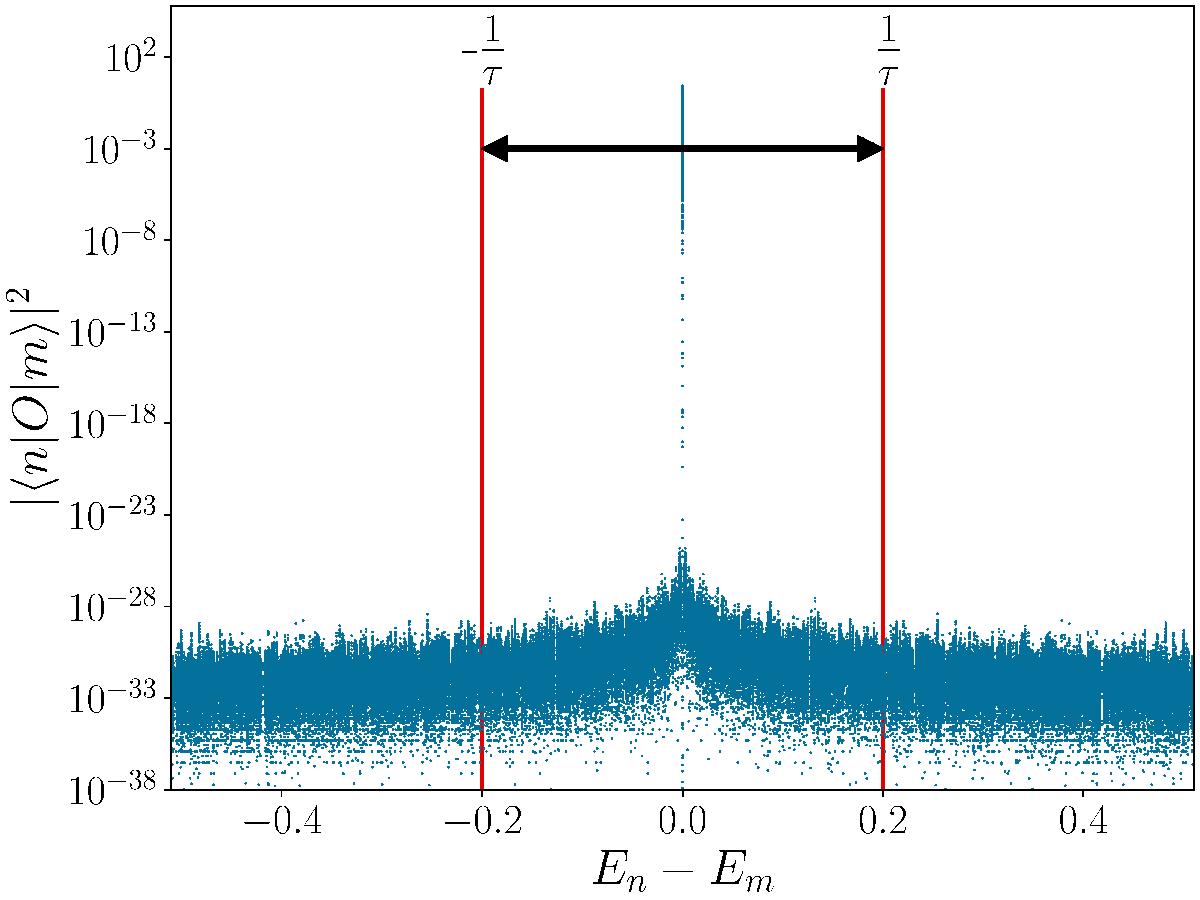
\includegraphics[width=0.5\textwidth]{Figures/cutoff_flat.pdf}
  \caption{Illustration of averaging procedure as defined by equation~\eqref{def:simple time avg}. The sum
  of matrix elements is restricted by the theta function to the region between the two red lines. In the case
  of operator shown here, we see that only the matrix elements corresponding to differences of energies
  very close to zero contribute to the time average. }
  \label{fig:cutoff}
\end{figure}


Observing that \({\left(\theta_{mn}^{\tau}\right)}^2 = \theta_{mn}^{\tau}\) and \({\left(\bar{A}^{\tau}\right)}_{mn} =
\theta_{mn}^{\tau} A_{mn}\) we can easily show some crucial properties of the time averaging:
\begin{proposition}
  For any \(A,B \in \mathcal{V}_L\)
  \begin{equation*}
    \hs{\bar{A}^{\tau}}{\bar{B}^{\tau}} = \hs{A}{\bar{B}^{\tau}} = \hs{\bar{A}^{\tau}}{B}
  \end{equation*}
  and
  \begin{equation*}
    \overline{\left(\bar{A}^{\tau}\right)}^{\tau} = \left(\bar{A}^{\tau}\right)
  \end{equation*}
  \label{prop:projection}
\end{proposition}

\begin{proof}
  \begin{align*}
    \hs{\bar{A}^{\tau}}{\bar{B}^{\tau}}  & = \frac{1}{\dimension} \sum_{mn} {\left(\bar{A}^{\tau}\right)}_{mn}
    {\left(\bar{B}^{\tau}\right)}_{mn}^{\ast} = \frac{1}{\dimension} \sum_{mn} {\left(\theta_{mn}^{\tau}\right)}^2 A_{mn} B_{mn}^{\ast} \nonumber{}               \\
    & = \frac{1}{\dimension} \sum_{mn} \left(\theta_{mn}^{\tau}\right) A_{mn} B_{mn}^{\ast} =
    \hs{A}{\bar{B}^{\tau}} = \hs{\bar{A}^{\tau}}{B}                                                                                                        \\
    \overline{\left(\bar{A}^{\tau}\right)}^{\tau} & = {\left(\theta_{mn}^{\tau}\right)}^2 A_{mn} = \theta_{mn}^{\tau} A_{mn} = \left(\bar{A}^{\tau}\right)
  \end{align*}
  
\end{proof}

These two facts reveal an interesting interpretation of the time averaging, namely that it can be
thought of as an orthogonal projection in vector space \(\mathcal{V}_L\). The involutive character of this operation explains,
why we can consider \(\bar{A}^{\tau}\) time independent in the time window \(\left(0,\tau\right)\).

Let us now calculate the commutator of time-averaged operator with the Hamiltonian:
\begin{align}
  \comm{H}{\bar{A}^{\tau}} & = \sum_n \sum_{k,p} E_n \theta_{kp}^{\tau} A_{kp} \comm{ \ketbra{n}{n}}{ \ketbra{k}{p}} \nonumber         \\
                           & = \sum_{k,p} \left(E_k-E_p\right) \theta_{kp}^{\tau} A_{kp} \ketbra{k}{p} \xrightarrow{\tau \to \infty} 0 \label{eq:time averaged commutator}
\end{align}
The last limit follows directly from equation~\eqref{eq:inf time avg}. We can see that the infinite time averaging procedure
creates an integral of motion, i.e. \(\comm{H}{\bar{A}} = 0\). Nonetheless, it is not enough to just time average a
local operator in order to get a local integral of motion, because in general \(A\in \mathcal{V}_L^M  \nRightarrow \bar{A} 
\in \mathcal{V}_L^M\), that is the truncation of matrix elements modifies the support of an operator.
One possible approach to checking its locality would be to
express this operator in the basis defined in~\eqref{eq:basis}. If for some \(M\) we have \(\bar{A}\in \mathcal{V}_L^M\),
then it is local. Second possibility is that it can be written as a convergent series of operators from \(\mathcal{V}_L^m\) with
increasing \(m\) --- then it is quasilocal. Otherwise it is a generic nonlocal quantity. But can we do better than this
direct approach?

To answer this question, we fix \(0\leq M \leq L/2\) and construct a basis \(\{O_s\}\) of \(\mathcal{V}_L^M\). How to actually perform such construction
will be shown in Section~\ref{sec:example}. Next, we find time averages of all basis operators and build a matrix
\begin{equation}
  K_{st}^{\tau} = \hs{\bar{O_s}^{\tau}}{\bar{O_t}^{\tau}}
  \label{eq:stiffness matrix}
\end{equation}
This matrix is Hermitian by design. However, the models we usually
consider posses time-reversal symmetry, and so we may assume that it is real and symmetric.
Therefore, the spectral theorem guarantees existence of an orthogonal matrix \(U\) that
diagonalizes it. In other words, \(D = UK^{\tau}U^{T}\) is diagonal and we have the following relations:
\begin{align}
  &\sum_{s, t} U_{n s} K_{s t}^{\tau} U_{t m}^{T}=\delta_{nm} \lambda_{n} \in \RR,\;\;\; \lambda_n \text{ --- eigenvalue of }K^{\tau} \nonumber \\
  &UU^{T} = U^{T}U = \mathbb{1} \implies \sum_{s} U_{ns}U_{sm}^{T} = \delta_{mn}\nonumber\\
  & U K = D U \implies \sum_s U_{ns} K_{st}^{\tau} = \sum_s  \delta_{ns} \lambda_s U_{st} = \lambda_n U_{nt}\label{eq:properties}
\end{align} 
With the help of the \(U\) matrix (eigenvectors of \(K^{\tau}\)) we can define a new set of rotated operators that
are time-independent in the window \(\left(0,\tau\right)\):
\begin{equation}
  Q_n = \sum_s U_{ns}\bar{O}_{s}^{\tau}\label{eq:new operators}
\end{equation} 

\begin{proposition}
Operators \(Q_n\) are orthogonal, i.e. \(\hs{Q_n}{Q_m} \propto \delta_{nm}\)
\label{prop:orthogonality}
\end{proposition}
\begin{proof}
  Let \(Q_n,Q_m\) be two operators defined as in~\eqref{eq:new operators}.
  Their orthogonality can be shown by direct calculation:
  \begin{align*}
    \hs{Q_n}{Q_m} &= \sum_{s,t} U_{ns} {\hs{\bar{O_s}^{\tau}}{\bar{O_t}^{\tau}}} U_{tm}^{T} 
    = \sum_{t} \left(\sum_{s}U_{ns} K_{st}^{\tau}\right)  U_{tm}^{T} \\ 
    &\triangleq \lambda_n \sum_t U_{nt} U_{tm}^{T} \triangleq \lambda_n \delta_{mn}
  \end{align*}
\end{proof}
The last two equalities, marked with \(\triangleq \), follow from properties~\eqref{eq:properties}. We can learn something more
about the eigenvalues of \(K^{\tau}\) matrix from a simple corollary to Proposition~\ref{prop:orthogonality}.
\begin{corollary}
  \(K^{\tau}\) is a positive semi-definite matrix.\label{corr:psd}
\end{corollary}
\begin{proof}
Let \(Q_n\) be defined as in~\eqref{eq:new operators}. Then, from the defining properties of inner product we have that
\(\hs{Q_n}{Q_n} \geq 0\). However, we also have that \(\hs{Q_n}{Q_n} = \lambda_n\). Combining these two equations, we get
that \(\left(\forall n\right) \left(\lambda_n \geq 0\right)\). Therefore \(K^{\tau}\) is a positive semi-definite matrix.
\end{proof}
This corollary provides us with a lower bound on spectrum of matrix \(K^{\tau}\). 

Let us now examine the support of \(Q_n\). By~\eqref{eq:basis} and making use of~Proposition~\ref{prop:projection}
and properties~\eqref{eq:properties}, we can decompose into a part supported on up to \(M\) sites and a nonlocal part:
\begin{align}
  Q_n &=  \sum_s \hs{O_s}{Q_n}O_s + Q_s^{\perp} = \sum_{s,t} U_{n t}\hs{O_{s}}{\bar{O}_{t}^{\tau}}
  O_{s}+Q_{n}^{\perp} \nonumber \\
  &= \sum_{s,t} U_{n t}\hs{\bar{O}_{s}^{\tau}}{\bar{O}_{t}^{\tau}} O_{s}+Q_{n}^{\perp}
  = \sum_{s,t} U_{n t}K_{ts} O_{s}+Q_{n}^{\perp} \nonumber \\
  &= \sum_s  \left( \sum_t U_{n t}K_{ts}^{\tau}\right) O_{s}+Q_{n}^{\perp} = \sum_{s} 
  \lambda_{n} U_{n s} O_{s}+Q_{n}^{\perp} = Q_{n}^{M}+Q_{n}^{\perp}
  \label{eq:decomposition}
\end{align}
Now we are ready to derive central result, stating why this actually algorithm works. Combining the fact that 
\(\hs{Q_n}{Q_n} = \lambda_n \)(see proof of Proposition~\ref{prop:orthogonality}) with~\eqref{eq:decomposition} we obtain:
\begin{align}
  \lambda_n &= \hs{Q_n}{Q_n} = \hs{Q_n^M + Q_n^{\perp}}{Q_n^M + Q_n^{\perp}} = \hs{Q_n^M}{Q_n^M} +
   \hs{Q_n^{\perp}}{Q_n^{\perp}} + \underbrace{2 \hs{Q_n^M}{Q_n^{\perp}}}_{=0 \text{ (cf.~\eqref{eq:basis})}} \nonumber \\
   &= \hs{\sum_s \lambda_n U_{ns} O_s}{\sum_t \lambda_n U_{nt} O_t} + \norm{Q_n^{\perp}}^2 =
  \lambda_n^2 \sum_{s,t} U_{ns} \hs{O_s}{O_t} U_{tn}^{T} + \norm{Q_n^{\perp}}^2  \nonumber \\
  &=\lambda_n^2 + \norm{Q_n^{\perp}}^2
\end{align}
Rearranging the above equality we get that \(\lambda_n - \lambda_n^2 = \norm{Q_n^{\perp}}^2 \geq 0\), which together with
Corollary~\ref{corr:psd} gives \(\lambda_n \in \left[0,1\right]\). 


From now on, we will focus on the case \(\tau \to \infty \), as it guarantees that \(\bar{O_s}\)'s and hence \(Q_n\)'s
commute with the Hamiltonian. 
Consequently, we finally arrive at a classification scheme for the support of \(Q_n\)'s.
\begin{definition}[Classification of IOMs]
  An integral of motion \(Q_n\) is called:
  \begin{itemize}
    \item local: \(\lambda_n = 1 \implies \norm{Q_n^{\perp}} = 0 \implies Q_n \in \mathcal{V}^M_L\)
    \item quasilocal: \(\lambda_n \in \left(0,1\right) \implies \norm{Q_n^{\perp}} > 0 \implies Q_n \in \mathcal{V}_L \)
    \item generic nonlocal: \(\lambda_n = 0 \implies \norm{Q_n} = 0\)
  \end{itemize}
  \label{def:classification}
\end{definition}
The procedure outlined above works for a fixed system size \(L\).
To asses the character of an integral of motion, we need to examine how \(\lambda_n\) 
behaves in the thermodynamic limit. To achieve this, we execute this algorithm for a 
few accessible values of \(L\) and then proceed with finite size scaling.
However, in this thesis we will examine both the \(L\to \infty \) case and \(L = 14\)
case, because that is largest system size for exact diagonalization that we were able to achieve.

It is important not to loose the physical interpretation of these results amidst all the formal development.
Operator \(Q_n = \sum_s U_{ns}\bar{O}_{s} = Q_n^M + Q_n^{\perp} \) is always an integral of motion, 
because it is a linear combination of infinite-time averaged operators (cf.~\eqref{eq:time averaged commutator}).
However, the time averaging procedure expands the support of initially local basis operators \(O_s\).
In actual computations we are using the basis of operators supported on up to \(M\) sites at all times, therefore the operators
obtained from the eigenvectors of \(K\) matrix are \(Q_n^M\) operators. If \(\lambda_n = 1\), then
\(\norm{Q_n^{\perp}} = 0 \implies Q_n^{\perp} = 0\) and \(Q_n = Q_n^M\). Therefore, \(Q_n^M\) operator, which
structure we know, is strictly conserved. On the other hand, if \(\lambda_n \in (0,1) \), then
\(\norm{Q_n^{\perp}} > 0 \implies Q_n^{\perp} \neq 0\) and \(Q_n \neq Q_n^M\). This means that the operator
that we really get from the algorithm is not a conserved quantity. It is an local approximation, or equivalently
a projection of true quasilocal integral of motion \(Q_n\) on a basis supported on up to \(M\) sites. Moreover, we can 
construct a convergent series of operators with increasing support and system size, such that their
norm approaches unity. In thermodynamic limit we obtain a strictly conserved
quantity that is \textit{quasilocal}. This discussion motivates a rather formal definition
of quasilocality~\autocite{zadnik2016,Prosen2014c}:
\begin{definition}
  An operator sequence \(\set{X_L}_{L\in \NN}\), \(X_L \in \mathrm{End}(\mathcal{H}^{\otimes L})\) which can be
  written as:
  \begin{equation*}
    X_L = \sum_{M\leq L} \sum_{i=0}^{L-1} \mathcal{S}^i (q_M \otimes \Id^{\otimes(L-r)})
  \end{equation*}
  where \(q_M \in \mathrm{End}(\mathcal{H}^{\otimes M})\) and there exist such constants \(\gamma, \zeta > 0 \) that
  \begin{equation*}
    \norm{q_M} \leq \gamma e^{-\zeta M}
  \end{equation*}
  is called \textit{quasilocal}.
  \label{def:formal quasilocal}
\end{definition}
In the above definition, \(\mathcal{H} = \mathbb{C}^2\) is the single spin Hilbert space,
\(\mathrm{End}(V)\) is the space of endomorphism on vector space \(V\), that is linear maps from \(V\) to \(V\)
and \(\mathcal{S}^i\) is the periodic left-shift operator defined as 
\begin{equation*}
  \mathcal{S}\left(\tau^{s_{0}} \otimes \tau^{s_{1}} \otimes \cdots 
  \tau^{s_{n-2}} \otimes \tau^{s_{n-1}}\right)=\tau^{s_{1}} \otimes
   \tau^{s_{2}} \otimes \cdots \tau^{s_{n-1}} \otimes \tau^{s_{0}}
\end{equation*}
However, in subsequent parts of this thesis we will use the Definition~\ref{def:classification}, while
keeping in mind its interpretation. We will end the discussion about the algorithm with 
a short summary on support of \(Q_n\):
\begin{align}
  & Q_n = Q_n^M + Q_n^{\perp}\nonumber\\
  & \norm{Q_n}^2 = \lambda_n \nonumber\\
  & \norm{Q_n^M}^2 = \lambda_n^2 \nonumber\\
  & \norm{Q_n^{\perp}}^2 = \lambda_n - \lambda_n^2
  \label{eq:summary of support}
\end{align}

\paragraph{Proof of corectness}
Suppose we have an operator \(\mathcal{V}_L^M \ni A = \sum_s u_s O_s \), where \(u_s \in \RR \) for all \(s\).
We can identify this operator from \(\mathcal{V}_L^M\) with a vector \( \vec{u} \in \RR^{\dim{\mathcal{V}_L^M}}\). Using this picture,
the stiffness of \(A\) can be calculated as follows:
\begin{equation}
  \hs{\bar{A}}{\bar{A}} = \sum_{s,t} u_s \hs{\bar{O}_s}{\bar{O}_t} u_t = \sum_{s,t} u_s K_{st} u_t = 
   \vec{u}^{T} K \vec{u}  
\end{equation} 
Thus, a problem in quantum mechanics is reduced to a problem in linear algebra.
Because all eigenvalues of \(K\) matrix are real, we can sort the corresponding operators (defined with columns of \(U\) matrix,
i.e.\;eigenvectors of \(K\)) by their magnitude. We then say that the larger the eigenvalue, the `better' the integral of motion is.
But can we be sure, that the maximal eigenvalue obtained from the algorithm corresponds to the `best' possible integral of motion?
To put it another way, if the procedure detects neither local nor quasilocal integrals of motion, does that necessarily mean they
do not exist for a given system? The answer to this question lies within the subsequent
\begin{proposition}
Let \(\lambda \) be the maximal eigenvalue of \(K\). Then the following equality holds:
\begin{equation*}
  \lambda = \max_{  \substack{\vec{v}\in \RR^{\dim{\mathcal{V}_L^M}}\\\norm{v} = 1}  }{\vec{v}^{T} K \vec{v}}
\end{equation*}
\end{proposition}
\begin{proof}
  Assume the converse, i.e. there exists such \(\vec{u} \in \RR^{\dim{\mathcal{V}_L^M}}\) that \(\vec{u}^T K \vec{u} > \lambda\)
  and \(\norm{u} = 1\).
  Let \(\{\vec{v}_n\}_n\) be a orthonormal basis consisting of eigenvectors of \(K\). We can express \(\vec{u}\) in this basis as
  \(\sum_n u_n \vec{v}_n\) for \(u_n \in \RR\). Then we have:
  \begin{align*}    
    \vec{u}^T K \vec{u} &= \left( \sum_n u_n \vec{v}_n^{T} \right) K  \left( \sum_m u_m \vec{v}_m \right) 
    = \sum_{n,m} u_n u_m \lambda_m \underbrace{\vec{v}_n^{T} \vec{v}_m}_{\delta_{mn}} \\
    &= \sum_n u_n^2 \lambda_n \leq \sum_n u_n^2 \lambda = \lambda \sum_n u_n^2 = \lambda   
  \end{align*}
  Obtained contradiction concludes the proof.
\end{proof}

%%%%%%%%%%%%%%%%%%%%%%%%%%%%%%%%%%%%%%%%%%%%%%%%%%%%%%%%%%%%%%%%%%%%%%%%%%%%%%%%%%%%%%%%%%%%%%%%%%%%%%%%%%%%%%%%%%%%%%%%%%%%%%%

\section{Spectral function and Mazur bound\label{sec:spectral function}}

\paragraph{Spectral function}After we have learned about local and quasilocal IOMs and how to find them, it is perhaps the 
time to ask why are they actually important? To answer this question in a convincing manner we 
will follow the discussion in~\textcite{Vidmar2021} and introduce the concept of spectral
functions. 

Suppose that we have an observable \(A \in \mathcal{V}_L^M\) and we are interested in studying its time
evolution. An obvious choice would be to calculate its autocorrelation function
\((A(t)|A)\), where the time dependence of \(A(t)\) is understood
via the Heisenberg picture i.e.\ \(A(t) = \exp\left(i H t\right) A
\exp\left(-i H t\right)\). However, this quantity is rather unpleasant to work with.
Instead, we will investigating the Fourier transform of autocorrelation function, formally
defined as:
\begin{definition}[Spectral function]  
  \begin{equation*}
  S(\omega) =  \lim _{\varepsilon \to 0^+} \frac{1}{2 \pi} \int_{-\infty}^{\infty} \mathrm{d} t 
  \; e^{i \omega t-|t| \varepsilon}\hs{A(t)}{A}
  \end{equation*}
  \label{def:spectral function}
\end{definition}
The limit in the definition is present in order to ensure proper convergence of the integral
and \(\omega{}\) corresponds to \(\frac{1}{\tau}\) from earlier discussion.
To connect this quantity with numerical calculations and to smoothen out any fluctuations, we
can once again integrate it, but this time over a finite frequency window:
\begin{equation}
  I(\omega) = \int_{-\omega}^{\omega} \mathrm{d}\omega' \; S(\omega') = 
  \frac{1}{\dimension} \sum_{m,n} \theta\left(\omega - |E_m-E_n|\right) A_{mn}^2
\end{equation}
It turns out that this quantity is equal to the square of Hilbert-Schmidt norm of time
averaged operator \(\bar{A}^{\frac{1}{\omega}}\), which fits nicely within the previously
discussed framework. Because all observables of interest are traceless and
normalized to unity, we have this two important limits
\begin{align}
  \lim_{\omega \to \infty } I(\omega) &= \frac{1}{\dimension}\sum_{m,n} A_{mn}^2 = \norm*{A}^2 = 1\\
  \lim_{\omega \to 0^+ } I(\omega) &= \frac{1}{\dimension} \sum_{ \substack{m,n\\E_m=E_n} } A_{mn}^2 = \norm*{\bar{A}}^2
\end{align}

For frequencies small (long times) in comparison with system's characteristic energy
scale, spectral function of an observable \(A \in \mathcal{V}_L^M\) attains the following approximation:
\begin{equation}
  S(\omega \ll  J) \simeq  D_{A} \delta(\omega)
  \label{eq:spectral approximation}
\end{equation}
where \(D_A = \lim_{\omega\to 0^+} I(\omega)\) is the stiffness of an observable.
Let us now imagine that we have a complete set of orthogonal (Q)LIOMs 
\(\hs{Q_{n}}{Q_{m}} \propto \delta_{nm}\). It was shown 
by~\textcite{Mazur1969,Suzuki1971} that the stiffness \(D_{A}\) of arbitrary observable \(A\) has its origin
in the projections on these \(Q_{n}\):
\begin{equation}
  D_A = \sum_{n} D_{n} = \sum_{n} \frac{\hs{A}{Q_{n}}^2}
  {\hs{Q_{n}}{Q_{n}}}
  \label{eq:mazur equality}
\end{equation}
Therefore, by calculating the overlap between our observable and all the (Q)LIOMs, we can infer about the long time
behavior of its spectral function and thus its autocorrelation function. It is here that the
importance of (Q)LIOMs becomes evident, as the overlap with generic nonlocal conserved quantities
vanishes in the thermodynamic limit~\autocite{Zotos1997}.
Because autocorrelation function of
LIOMs is constant, its Fourier transform is a Dirac delta, which explains the form of 
equation~\eqref{eq:spectral approximation}. 

\paragraph{Mazur bound} If we know only a subset of the full set of (Q)LIOMs, this equality turns into 
a very useful lower bound for stiffness, called the \textit{Mazur bound}. We will now proceed with a derivation
of this bound for the case of one (Q)LIOM, in the spirit of a more modern discussion from~\textcite{Ilievski2016a}.
\begin{proposition}[Mazur bound for a single (Q)LIOM]
  Let \(A\in \mathcal{V}_L^M\) be an arbitrary observable and \(Q\) be a (quasi)local conserved quantity. Then the following inequality
  holds:
  \begin{equation*}
    D_{A} = \hs{\bar{A}}{\bar{A}} \geq \frac{\hs{A}{Q}^2}{\hs{Q}{Q}}
  \end{equation*}
  \label{prop:single mazur}
\end{proposition}

\begin{proof}
  We define a new observable \(\mathcal{A} = \bar{A} - \alpha Q\) for \(\alpha \in \RR\).
  Obviously, square of the norm of this quantity is positive i.e. \(\norm*{\mathcal{A}}^2 = 
  \tr(\mathcal{A}\mathcal{A})/\dimension \geq 0\). On the other hand, we can carry out an
  explicit computation of the norm:
  \begin{align*}
  \norm*{\mathcal{A}}^2 &= \hs{\bar{A}-\alpha Q}{\bar{A}-\alpha Q} = \hs{\bar{A}}{\bar{A}} - 
  \hs{\bar{A}}{Q} - \alpha \hs{Q}{\bar{A}} + \alpha^2 \hs{Q}{Q} \\
  &= \hs{\bar{A}}{\bar{A}} - 2\alpha \hs{A}{Q} + \alpha^2 \hs{Q}{Q} \geq 0
  \end{align*}
  Between the first and the second line we have used the fact that \(\hs{\bar{A}}{\bar{B}} = 
  \hs{\bar{A}}{B} = \hs{A}{\bar{B}}\)(cf. Proposition~\ref{prop:projection}) and \(\bar{Q} = Q\) 
  for a conserved quantity. Let us now substitute \(\alpha = \frac{\hs{A}{Q}}{\hs{Q}{Q}}\) to the
  above inequality.
  \begin{align*}
    D_A = \hs{\bar{A}}{\bar{A}} &\geq 2 \frac{\hs{A}{Q}}{\hs{Q}{Q}} \hs{A}{Q} - \frac{\hs{A}{Q}^2}{\hs{Q}{Q}^2}\hs{Q}{Q}
    = \frac{\hs{A}{Q}^2}{\hs{Q}{Q}}
  \end{align*}
  \label{proof:single mazur}  
\end{proof}
It is perhaps worth noting, that the derivation Mazur bound for a single (Q)LIOM is almost equivalent to the proof of
the Cauchy-Schwarz inequality, found in any linear algebra textbook. By following exactly the same procedure, 
we can easily generalize this results to a set of orthogonal conserved quantities \(\{Q_{n}\}\):
\begin{equation}
  D_A = \hs{\bar{A}}{\bar{A}} \geq \sum_{n} \frac{\hs{A}{Q_n}^2}{\hs{Q_n}{Q_n}}
\end{equation}

We have already seen that Mazur inequality turns into an equality, if the set \(\{Q_n\}\) is complete. However,
up until a few years ago, it was not clear how to systematically identify such a complete set in interacting models.
This have changed with the work of~\textcite{Mierzejewski2015a}, where the algorithm described in details
in Section~\ref{sec:algorithm} was first proposed. We will now show that the following proposition holds:

\begin{proposition}[Saturation of Mazur bound]
  The set \(\{Q_n\}\) of (Q)LIOMs obtained from the algorithm in Section~\ref{sec:algorithm} is complete,
  that is it saturates the Mazur bound. 
\label{prop:saturation}
\end{proposition}
\begin{proof}
  Consider once again an arbitrary observable \(\mathcal{V}_L^M \ni A = \sum_n a_n O_n,\; 
  (\forall n) (a_n \in \RR)\). We are interested in computing its stiffness \(D_A = \hs{\bar{A}}{\bar{A}}\), 
  where \(\bar{A} = \sum_n a_n \bar{O}_n\). Inverting the relation~\eqref{eq:new operators}, we can write 
  \(\bar{O_n} = \sum_s U_{ns}^T Q_s = \sum_s U_{sn} Q_s\) and thus the following:
  \begin{equation*}
    \bar{A} = \sum_n a_n \bar{O}_n = \sum_n a_n \sum_s U_{sn} Q_s =
    \sum_s \underbrace{\left(\sum_n a_n U_{sn}\right)}_{v_s} Q_s = \sum_s v_s Q_s
  \end{equation*}
  Now, let us express the overlap \(\hs{\bar{A}}{Q_k}\) in two ways:
  \begin{enumerate}
    \item \(\hs{\bar{A}}{Q_k} = \sum_s v_s \underbrace{\hs{Q_s}{Q_k}}_{=\lambda_s \delta_{sk}} = v_k \lambda_k\)
    \item \(\hs{\bar{A}}{Q_k} = \hs{A}{\bar{Q_k}} = \hs{A}{Q_k}\)
  \end{enumerate}
  We are finally ready to make a direct calculation of stiffness of \(A\):
  \begin{align*}
    D_A = \hs{\bar{A}}{\bar{A}} &= \sum_{sk} v_s v_k \hs{Q_s}{Q_k} = \sum_{sk} v_s v_k \delta_{sk} \lambda_{k} = 
    \sum_{\substack{s\\\lambda_s > 0}} v_s^2 \lambda_s \\
    &= \sum_{\substack{s\\\lambda_s > 0}} v_s^2 \lambda_s^2 \frac{1}{\lambda_s} = 
    \sum_{\substack{s\\\lambda_s > 0}} \frac{\hs{A}{Q_s}^2}{\hs{Q_s}{Q_s}}
  \end{align*}
  Therefore, the Mazur bound is saturated by our construction and the proof is concluded.
\end{proof}
We will finish the section with an example of an application of Mazur bound. 
\begin{example}
  We consider the topic of ballistic linear response~\autocite{Ilievski2016a}. Let \(J\) be an extensive current,
  for example the spin current. From Kubo linear response theory
  we have the following well-known expression for the real (non-dissipative) part of dynamical
  spin conductivity~\autocite{Zotos1996}:
  \begin{equation}
    \sigma'(\omega) = 2 \pi D_J \delta(\omega) + \sigma_J^{reg}(\omega)
  \label{eq:conductivity}
  \end{equation}
If there exists a (quasi)local conserved quantity \(Q\) such that \(\hs{J}{Q}>0\), the Mazur bound
implies that \(D_J > 0\). Such nonzero value of spin current stiffness is an indicator of \textit{ballistic}
DC transport (i.e.\ without scattering, cf. Figure~\ref{fig:spin transport}) --- \(\sigma'(0)\) diverges. 
\end{example}
\begin{figure}[htbp]
  \centering
  \begin{tikzpicture}[scale=1.4]
    \colorlet{col1}{blue!30}
  
   \begin{scope}[smooth,draw=gray!20,y=0.3989422804cm]
        \filldraw[fill=col1] plot[id=f1, domain=-1.5:1.5,samples=100] function {6*exp(-6*x*x)};
        \draw[black] plot[id=f2,domain=-1.5:1.5,samples=100]
            function {6*exp(-6*x*x)};
    \end{scope}
    \draw[->] (-1.5,0) -- (1.5,0) node [right] {$x$};
    \draw[->] (-1.5,0) -- (-1.5,2.5) node [midway,rotate=90,yshift=6pt] {spin density};
    \draw[<->] (-0.37,1) -- (0.37,1) node [midway, yshift=6pt] {$\gamma$};
  
    \begin{scope}[smooth,draw=gray!20,y=0.3989422804cm]  
      \draw[black] plot[id=f3,domain=2.35:5.35,samples=100] function {0.7};    
      \draw[black] plot[id=f4,domain=2.35:5.35,samples=100] function {x};    
      \draw[black] plot[id=f5,domain=2.35:5.35,samples=100] function {sqrt(x)};    
    \end{scope}  
    
    \draw[->] (2.35,0) -- (5.35,0) node [right] {$t$};
    \draw[->] (2.35,0) -- (2.35,2.5) node [right] {$\gamma$};
    \node[draw=none] at (3.35,1.6) {$\gamma \propto t$};
    \node[draw=none] at (3.45,0.95) {$\gamma \propto \sqrt{t}$};
    \node[draw=none] at (3.6,0.4) {$\gamma = const$};
    \node[draw=none] (localized) at (6,0.3) {localized};
    \node[draw=none,above of=localized,node distance=27pt] (diffusive) {diffusive};
    \node[draw=none,above of=diffusive,node distance=45pt] (ballistic) {ballistic};
  \end{tikzpicture}  
  \caption{Illustration of different types of transport. On the left panel, we have some initial spin
  density characterized by width \(\gamma\). On the right panel, we have the dependence of \(\gamma\)
  on time in three different cases.}
  \label{fig:spin transport}
\end{figure}

%%%%%%%%%%%%%%%%%%%%%%%%%%%%%%%%%%%%%%%%%%%%%%%%%%%%%%%%%%%%%%%%%%%%%%%%%%%%%%%%%%%%%%%%%%%%%%%%%%%%%%%%%%%%%%%%%%%%%%%%%%%%%%%%

\section{(Q)LIOMs supported on up to \(3\) sites in the XXZ model\label{sec:example}}

After explaining how and why to look for LIOMs and QLIOMs, let us now turn to a more concrete
example of spin-\(1/2\) XXZ model on one dimensional lattice of \(L\) sites with periodic
boundary conditions, introduced already in Section~\ref{sec:xxz}. In the subsequent
considerations we will base on the work of~\textcite{Mierzejewski2015a}.

Having chosen a concrete model, we can now give an explicit definition of a basis
of a space of \(m\)-local observables \(\mathcal{V}_L^m\). It is composed of operators
of the form:
\begin{equation}
  O_{\underline{s},j}=\sigma_{j}^{s_{1}} \sigma_{j+1}^{s_{2}} \cdots 
  \sigma_{j+m-1}^{s_{m}}
  \label{eq:basis operator}
\end{equation}
In the expression above we have \(\sigma_j^z \equiv 2 S^z_j\),
\(\sigma_j^{\pm} \equiv \sqrt{2} S_j^{\pm}\), \(\sigma^{0}_j \equiv \Id_{2\cross 2}\) and
 \(\underline{s} = \left(s_1, s_2,\ldots, s_m\right)\) where \(s_j \in \{+,-,z,0\}\) for
 \(j \in \{2,3,\ldots,m-1\}\). For first and last operator in a sequence we have 
 \(s_{1,m} \in \{+,-,z\}\), because an identity there would correspond to an \(m-1\)-local
 operator. The index \(j\) indicates first site of the support.
As a matter of mathematical precision, the notation for \(O_{\underline{s},j}\) used here 
(and frequently in physics literature) is a bit of simplification. It is important to remember
that implicitly, there are tensor products between \(\sigma_j\)'s, i.e.\ we have the following:
\begin{equation}
  O_{\underline{s},j}= \underbrace{\Id_{2\cross 2} \otimes \cdots
       \otimes \Id_{2\cross 2}}_{j-1} \otimes \; \sigma_{j}^{s_{1}} \otimes \sigma_{j+1}^{s_{2}} \otimes
        \cdots \otimes \sigma_{j+m-1}^{s_{m}} \otimes 
        \underbrace{\Id_{2\cross 2} \otimes \cdots \otimes \Id_{2\cross 2}}_{L-j-m+1}
        \label{eq:basis with tensors}
\end{equation}
The single site identity operators ensure that the dimension of matrix of the operator is right.
A simple combinatorial observation shows us, that there are \(N_m = 3\cdot 4^{m-2}\cdot 2\)
(excluding shifts i.e.\ different values of \(j\) for the same \(\underline{s}\)) operators
constituting a \(m\)-local basis (for \(m = 1\) we have \(N_1 = 3\)). Moreover, they are orthonormal
\textit{by design}, i.e.\ \(\hs{O_{\underline{s},j}}{O_{\underline{s}^{\prime}},j^{\prime}} =
\delta_{\underline{s},\underline{s}^{\prime}}\delta_{j,j^{\prime}}\) (see Appendix~\ref{app:orthonormality} for proof).
Fixing \(M>0\) (usually \(M<L\)), we can construct the basis of traceless operators spanning
the space \(\mathcal{V}_L^M = \bigoplus_{m=1}^{M} \mathcal{V}_L^m\). From the properties of 
direct sum of linear spaces we now that its cardinality is \(D_M = \sum_{m=1}^{M} N_m = 
 3 \cdot 4^{M-1}\). To include all possible shifts, this value needs to multiplied by
 the number of sites \(L\). Such construction can be implemented in practice by considering
 all possible \(M\)-digit numbers written in base \(4\) (as there are \(4\) `building blocks':
  \(\sigma^{\pm},\sigma^{z},\Id{}\)). 

Having put together this basis, we can now proceed with the rest of the (Q)LIOM finding algorithm.
However, before that it is beneficial to discuss the influence of symmetries of system in question,
the XXZ model. They allow us to decompose the matrix \(K\) 
(cf.~\eqref{eq:stiffness matrix}) and thus reduce the computational effort. First and perhaps
the most important one is implied by the fact already discussed in Section~\ref{sec:prelim} ---
conservation of magnetization. We could restrict our considerations to a subspaces
of \(\mathcal{V}_L^M\) comprised of operators such that \(\comm{S_{tot}^z}{O_{\underline{s}}} = 0\).
Yet, we will not be able to make use of that symmetry here, as in this work we are interested 
in the \textit{noncommuting} operators, i.e\ precisely those that break this symmetry.
Furthermore, the XXZ model is time-reversal invariant, so the \(K\) matrix is real and symmetric.
Therefore, we can divide our operators into two orthogonal subspaces, either real or imaginary.
Those subspaces are then spanned by operators of the form 
\(O_{\underline{s}}+O^{\dagger}_{\underline{s}}\) or 
\(i(O_{\underline{s}}-O^{\dagger}_{\underline{s}})\) respectively. There is also one more
useful symmetry, namely the \(\ZZ_2\) spin-flip symmetry, however it remains out scope of
this thesis. 


%%%%%%%%%%%%%%%%%%%%%%%%%%%%%%%%%%%%%%%%%%%%%%%%%%%%%%%%%%%%%%%%%%%%%%%%%%%%%%%%%%%%%%%%%%%%%%%%%%%%%%%%%%%%%%%%%%%%%%%%%%%%%%%%
\subsection{Commuting LIOM: Spin energy current\label{sec:energy current}}
In order to test our (Q)LIOM finding algorithm and the correctness of its implementation, we investigate the known case of
energy current in Spin\(-1/2\) XXZ model~\autocite*{Mierzejewski2015Approx} and see whether it is detected or not.
For the sake of completeness, derivation of
spin energy current for the general XYZ model will be presented, following the definitions in \textcite{Zotos1997}.
We start with the general XYZ Hamiltonian with periodic boundary conditions:
\begin{equation}
  H_{XYZ} = \sum_{k=1}^L  \left( J_{x} \Sx_{k}\Sx_{k+1} + J_{x} \Sy_{k}\Sy_{k+1} + J_{z} \Sz_{k}\Sz_{k+1} \right)
\end{equation}
It is easy to see that this Hamiltonian can be represented as a sum of operators supported on two consecutive sites:
\begin{equation}
  H_{XYZ} = \sum_{k=1}^L h_{k,k+1}
\end{equation}
where \(h_{k,k+1} = J_{x} \Sx_{k}\Sx_{k+1} + J_{x} \Sy_{k}\Sy_{k+1} + J_{z} \Sz_{k}\Sz_{k+1} \) and periodic boundary conditions
require that \(h_{L,L+1} = h_{L,1}\). The energy operator is a conserved quantity, thus the time evolution of its local density
is given by the discrete continuity equation:
\begin{equation}
  \dv{h_{k,k+1}(t)}{t} + \div{j_{k}^{E}(t)} = 0
  \label{eq:discrete continuity}
\end{equation}
where \(\div{j_{k}^E(t)} \equiv j_{k+1}^E(t) - j_{k}^E(t)\) is the discrete divergence of spin energy current density and \(h_{i,i+1}(t) = e^{i H_{XYZ}t} h_{i,i+1} e^{-i H_{XYZ} t}\).
On the other hand, time evolution of an arbitrary operator is determined
by the Heisenberg equations:
\begin{equation}
  \dv{h_{k,k+1}(t)}{t} = i \comm{H_{XYZ}}{h_{k,k+1}(t)}
  \label{eq:heisenberg equation}
\end{equation}
Combining equations~\eqref{eq:discrete continuity} and~\eqref{eq:heisenberg equation} we obtain the defining equations for
the spin energy current density:
\begin{equation}
  j_{k+1}^E - j_{k}^E = - i \comm{H_{XYZ}}{h_{k,k+1}} = i \comm{h_{k,k+1}}{H_{XYZ}} = i \sum_{r=1}^L \comm{h_{k,k+1}}{h_{r,r+1}}
  \label{eq:energy current defining equation}
\end{equation}
Similar equations can be written for any operator being a sum of local operators such as
the total spin operator or particle number operator in fermionic models. Detailed solution to equation~\eqref{eq:energy current defining equation}
is shown in Appendix~\ref{app:spin energy current derivation}. For the XXZ model we get the following expression:
\begin{align*}
  j_k^E & = i \Big( \underbrace{2J \Sm_{k-1}\Sz_k \Sp_{k+1} + J \Delta \Sz_{k-1}\Sp_k \Sm_{k+1} + J\Delta \Sp_{k-1}\Sm_k\Sz_{k+1}}_{O_k}                                  \\
        & - \underbrace{\left(2J \Sp_{k-1}\Sz_k \Sm_{k+1} + J\Delta \Sz_{k-1}\Sm_k \Sp_{k+1} + J\Delta \Sm_{k-1}\Sp_{k} \Sz_{k+1} \right)}_{O_k^{\dagger}}\Big) \nonumber \\
        & = i\left(O_k - O_k^{\dagger}\right)
\end{align*}
Thus we see that it is an imaginary operator.
Obtaining the energy current operator is now simply the matter of summing over all the lattice sites:
\begin{equation}
  J^E = \sum_{k=1}^L j_k^E
  \label{eq:energy current}
\end{equation}
As the energy current commutes with the Hamiltonian~\autocite{Zotos1997}, it does not undergo time evolution
and its autocorrelation function \(\hs{J^E(t)}{J^E(0)}\) is constant. Therefore, the corresponding
spectral function is proportional to Dirac delta.
\begin{figure}[htbp]
  \centering
  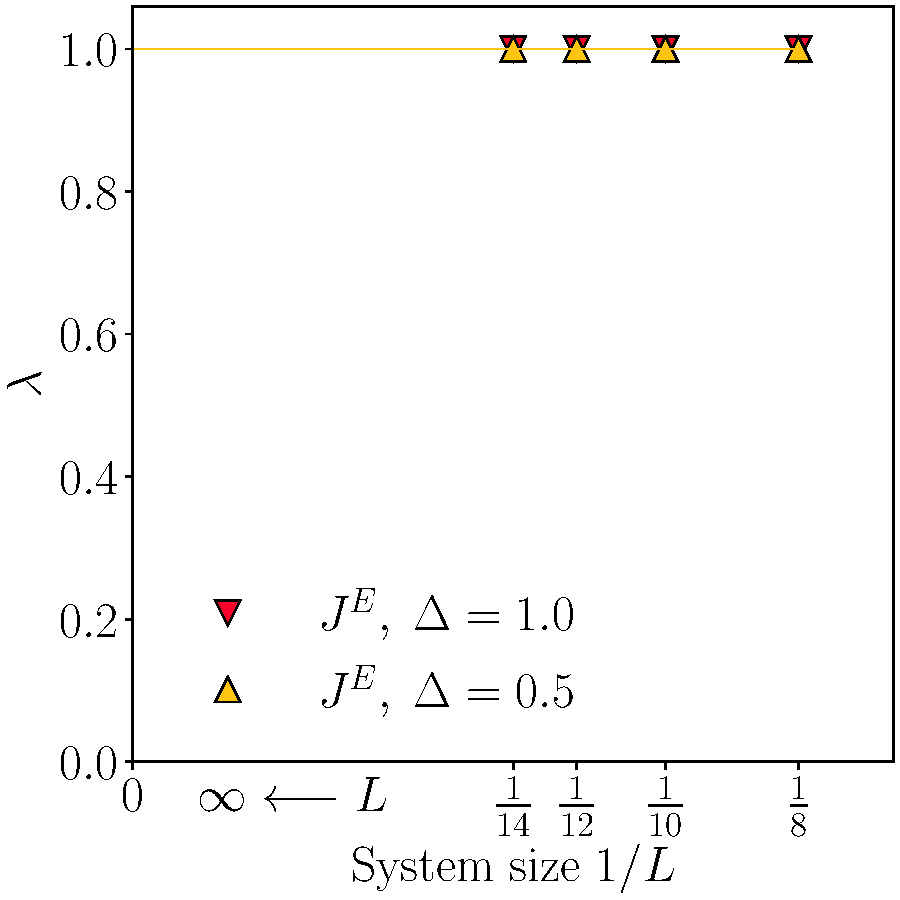
\includegraphics[width=0.5\textwidth]{Figures/current_int.pdf}
  \caption{Eigenvalues of generalized stiffness matrix corresponding to the energy current
  operator as a function of inverse system size. Solid line is the extrapolation to thermodynamic
  limit. Calculations performed for \(\Delta=1.0\) and \(\Delta=0.5\).}\label{fig: current integrable}
\end{figure}
After restricting our algorithm to the case of imaginary
operators, we obtain the following:
\begin{equation}
    J^E = \sum_{i=k}^L i\left[\beta_1 \left(\Sm_{k-1}\Sz_{k}\Sp_{k+1}\right) + \beta_2 \left(\Sz_{k-1}\Sp_{k}\Sm_{k+1}+\Sp_{k-1}\Sm_{k}\Sz_{k+1}\right)\right] + \text{H.c.}
\end{equation}
where the coefficients \(\beta_1,\beta_2\) are such that the operator is properly
normalized. This is precisely the energy current operator as derived above.
After taking the thermodynamic limit of the eigenvalue of \(K\) matrix 
corresponding to the energy current, we see that it equals one (Figure~\ref{fig: current integrable}).
Thus, according to Definition~\ref{def:classification}, it is a local integral of motion. 

%%%%%%%%%%%%%%%%%%%%%%%%%%%%%%%%%%%%%%%%%%%%%%%%%%%%%%%%%%%%%%%%%%%%%%%%%%%%%%%%%%%%%%%%%%%%%%%%%%%
\subsection{Noncommuting (Q)LIOMs}
Having checked the correctness of the algorithm and its implementation, we can now proceed with the
main topic of this thesis, that is investigating the \textit{noncommuting} integrals of motion. 
We conducted preliminary studies for small values of system size \(L\), without assuming
translational invariance. Available resources allowed us to make unrestricted search for
 \(L \in \set{8,9,10,11,12}\). Nevertheless, noncommuting operators that maximized stiffness for given 
 \(L\) and \(\Delta \) turned out to be either translationally invariant or translationally invariant with
 a sign flip (see \(\hat{O}_2\)~\eqref{eq:delta 0.5}). Therefore, we restrict our further 
considerations to such operators only. This allowed us to obtain numerical
results for \(L\) up to \(14\). We will focus on two concrete cases of operators, corresponding
to largest eigenvalues of generalized stiffness matrix for values of anisotropy
parameter \(\Delta=1.0\) and \(\Delta=0.5\) respectively. For this values of
\( \Delta \) parameter, the many-body energy spectra exhibits massive degeneracies, because
eigenstates with different \(\Sz_{tot}\) correspond to the same energies~\autocite{Fagotti2014,Mierzejewski2021}.

For the case of \(\Delta=1.0\), the XXZ model reduces to the isotropic Heisenberg model possessing full
\(SU(2)\) symmetry:
\begin{equation}
  H = J \sum_{i=1}^L \left(\Sx_i \Sx_{i+1} + \Sy_i \Sy_{i+1} + \Sz_i \Sz_{i+1}\right)
\end{equation}
As a consequence of this symmetry, conservation of total magnetization 
(\(\Sz_{tot}\) operator~\eqref{eq:magnetization}) implies the conservation of analogously defined \(\Sx_{tot}\)
and \(\Sy_{tot}\) and therefore the following quantity:
\begin{equation}
    \hat{O}_{1} =  \frac{1}{\sqrt{L}}\sum_{i=1}^{L} \Sp_{i} + \text{H.c.}
    \label{eq:delta 1.0}
\end{equation}
where the prefactor is introduced for the sake of normalization. Note that
this operator is actually the \(\Sx_{tot}\), however this form shows that \(\hat{O}_1\) 
is an example of a real operator. If we were to consider analogously defined imaginary operator,
we would obtain the \(\Sy_{tot}\), but due to \(SU(2)\) symmetry the results would be the same.


The case of \(\Delta=0.5\) is much more difficult. It was shown by~\textcite{zadnik2016} that for 
special values of anisotropy parameter \(\Delta \in S = \set[\Big]{\cos\left(\frac{2l}{2k-1}
\pi\right)}_{k,l\in \NN,\, l<k}\) one can use semicyclic irreducible representations
of quantum group \(U_q(\mathfrak{sl}_2)\) to generate a set of quasilocal integrals of 
motion that do not preserve magnetization. Even though the set \(S\) is a dense subset
of the interval \([-1,1]\) i.e.\ the gapless regime of XXZ spin-\(1/2\) chain, it is not
symmetric with respect to \(\Delta=0\). For example, considered here value of anisotropy parameter
\(\Delta=0.5\) does not belong to this set, whereas \(\Delta=-0.5\) do. However, it can be shown
that for even system sizes, in thermodynamic limit, there exist an unitary operator 
\(U = \left(\Id_{2\cross 2}\otimes \tau^z\right)^{\otimes L/2}\), which action is equivalent to flipping the sign 
of parameter \(\Delta\), that is \(UH_{XXZ}(\Delta)U = -H_{XXZ}(-\Delta)\). From that follows,
that if \(Q\) is a conserved quantity for \(\Delta\), then \(\tilde{Q} = UQU\) is a conserved
quantity for \(-\Delta\). This the reason why we present numerical results only for even 
values of \(L\). For \(\Delta=0.5\) the actions
of this operator produces a simple factor of \((-1)^i\) and the operator of interest reads:
\begin{equation}
  \hat{O}_{2} =\frac{1}{\sqrt{L}} \sum_{i=1}^{L} {(-1)}^i \left( \Sp_{i}\Sp_{i+1}\Sp_{i+2}\right) + \text{H.c.}
  \label{eq:delta 0.5}
\end{equation}  
This is once again a real operator. Detailed discussed of this topic is far beyond the scope of this thesis
and can be found in~\autocite{zadnik2016,Prosen2014c}.

\begin{figure}[htbp]
  \centering
  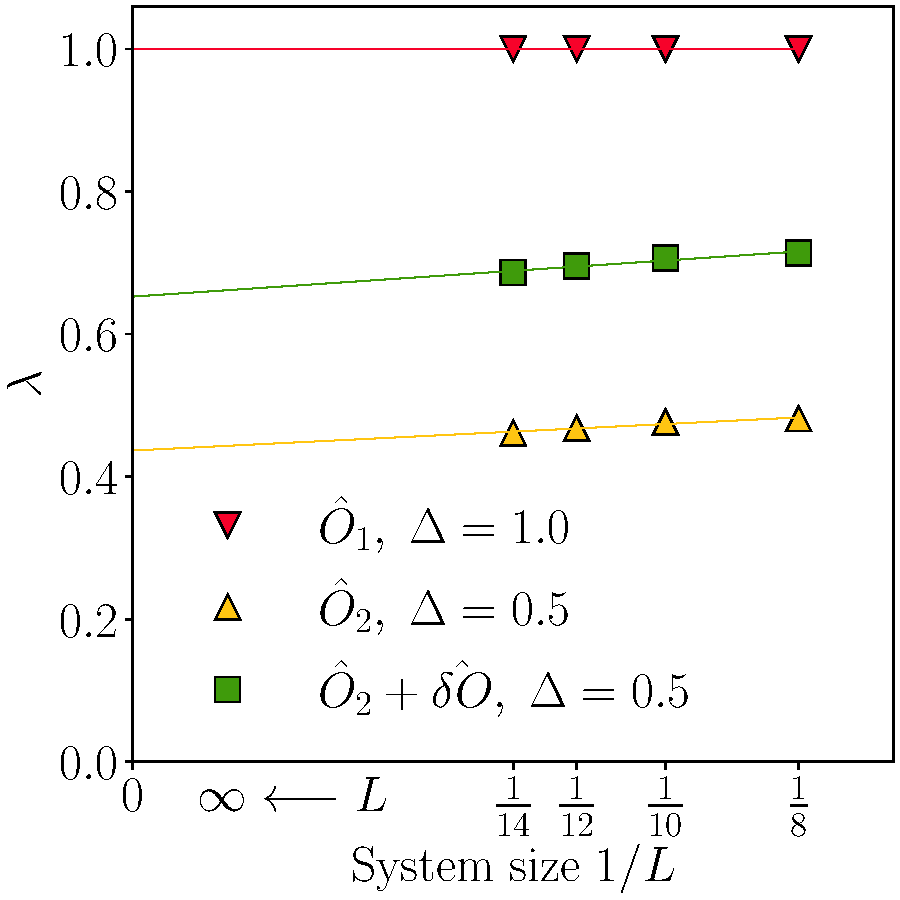
\includegraphics[width=0.5\textwidth]{Figures/nocomm_int.pdf}
  \caption{Eigenvalues of generalized stiffness matrix corresponding to the two noncommuting
    integrals of motion, as a function of inverse system size. Solid lines represent the extrapolation
    to the thermodynamic limit. Note that the operator \(\hat{O}_2\) exhibits quasilocality
    and its stiffness in the thermodynamic limit is \(\lambda_{L\to\infty} \approx
    0.44\). Stiffness of \(\hat{O}_2 + \hat{\delta O}\) in thermodynamic limit is
    \(\lambda_{L\to\infty} \approx 0.65\)}
  \label{fig: noncommuting integrable}
\end{figure}

Both \(\hat{O}_1\) and \(\hat{O}_2\) are noncommuting operators, what can be seen easily from the
fact that they consist of products of either just \(\Sp\) operators or \(\Sm\) operators. Conducting
an analysis with the help of the algorithm we indeed find these two operators among eigenvectors
of the generalized stiffness matrix. Corresponding eigenvalues and their thermodynamic limit
are shown in Figure~\ref{fig: noncommuting integrable}. Comparing it with 
Definition~\ref{def:classification} we see that \(\hat{O}_1\) is a strictly 
conserved, local integral of motion, whereas \(\hat{O}_2\) is a projection 
of a quasilocal integral of motion on a basis supported on up to \(3\) sites.
To further illustrate the concept of quasilocality, we can consider a projection
of this QLIOM on a basis supported on up to \(4\) sites, which results in an operator of the form 
\(\hat{O}_2 + \hat{\delta O}\), where \(\hat{\delta O}\) is the complicated \(4\)-local part,
which exact form is not important. Looking at Figure~\ref{fig: noncommuting integrable} we see
that stiffness of this new projection is larger that the old one. However, contribution 
of \(\hat{\delta O}\) to the overall stiffness is smaller than that of \(\hat{O_2}\), which
is in agreement with Definition~\ref{def:formal quasilocal}.

	\cleardoublepage{}

	\chapter{Relaxation of integrals of motions in weakly perturbed XXZ model}
\thispagestyle{chapterBeginStyle}

So far we have focused on investigating properties of an \emph{integrable} XXZ
spin-\(1/2\) chain. However, integrability is not a common property in the quantum world.
Many system requires fine-tuning of their parameters to achieve this, with perhaps a single
exception given by systems exhibiting many-body localization. Furthermore, we usually
do not have precise enough control over real-world systems to perform such fine tuning,
so full integrability is rarely seen (albeit some signatures of it were 
observed in an experiment~\autocite{Khemani2019}). It is thus desirable to investigate
 \emph{almost} integrable system, where the integrability-breaking perturbation is small.

Methodology in this chapter follows the work of~\textcite{Mierzejewski2015Approx},
however the results about relaxation of noncommuting integrals
of motion are original and at the moment of writing this thesis not found elsewhere
in literature. 
\section{Adding perturbation to the Hamiltonian}
We are now going to weakly break integrability of XXZ model~\eqref{eq:XXZ} 
by adding a perturbation in form of next-nearest neighbor interaction.
New Hamiltonian has the following form:
\begin{equation}
    H_{XXZ} = \frac{1}{2}\sum_{j = 1}^{L}\left( S^{+}_{j} S^{-}_{j+1} + 
    S^{-}_{j}S^{+}_{j+1} \right) + \Delta\sum_{j = 1}^{L} S^{z}_{j}S^{z}_{j+1}
    + \alpha H^{\prime}
    \label{eq:HXXZ perturbed}
\end{equation}
where \(H'\) is the perturbation that breaks integrability for nonzero \(\alpha \):
\begin{equation}
    H^{\prime}=\sum_{j = 1}^{L} S^{z}_{j}S^{z}_{j+2}
    \label{eq:perturbation}
\end{equation}
In such system, only two conserved quantities remain --- the Hamiltonian \(H_{XXZ}\) itself 
and the total magnetization \(\Sz_{tot}\). All other integrals of motions cease to be conserved
and decay with a finite relaxation time \(\tau\) (cf. Figure~\refeq{fig:cutoff}).
We are interested in investigating this decay and the timescales involved.
To this end we take the previously discussed (Q)LIOMs \(J^E, \hat{O}_1,\hat{O}_2\)
and examine their behavior under finite-time averaging 
(as defined in~\eqref{def:simple time avg}) generated by perturbed Hamiltonian.
As an initial check, we calculate the finite-time autocorrelation function (finite-time stiffness)
\(\lambda^{\tau}_A = \hs{\bar{A}^{\tau}}{\bar{A}^{\tau}}\) as a function of inverse system size.
In order to relate this to the discussion of spectral functions in Section~\ref{sec:spectral function},
we will from now on use the cutoff frequency \(\omega = \frac{1}{\tau}\), instead of the time of
averaging \(\tau\). The perturbation should be strong enough, that in the thermodynamic limit
\(\omega \to 0^+\) stiffness vanishes. Results are shown in Figure~\ref{fig:current decay}.
We see first hints that the behavior under perturbation for commuting and noncommuting operators
differ. For perturbation strength \(\alpha=0.2\) energy current stiffness does
not decay in thermodynamic limit for \(\omega \to O^+\) and thus stronger perturbation is needed.
However, stiffness of operators \(\hat{O}_1,\hat{O}_2\) vanish even for finite size systems
and smaller perturbations. \textcolor{blue}{Does this make sense? (d)-(i) Increasing nature of
stiffness is caused by \(\omega\) resolution smaller than energy levels spacings? Leave this or
delete this?}.
\begin{figure}[htbp]
  \centering
  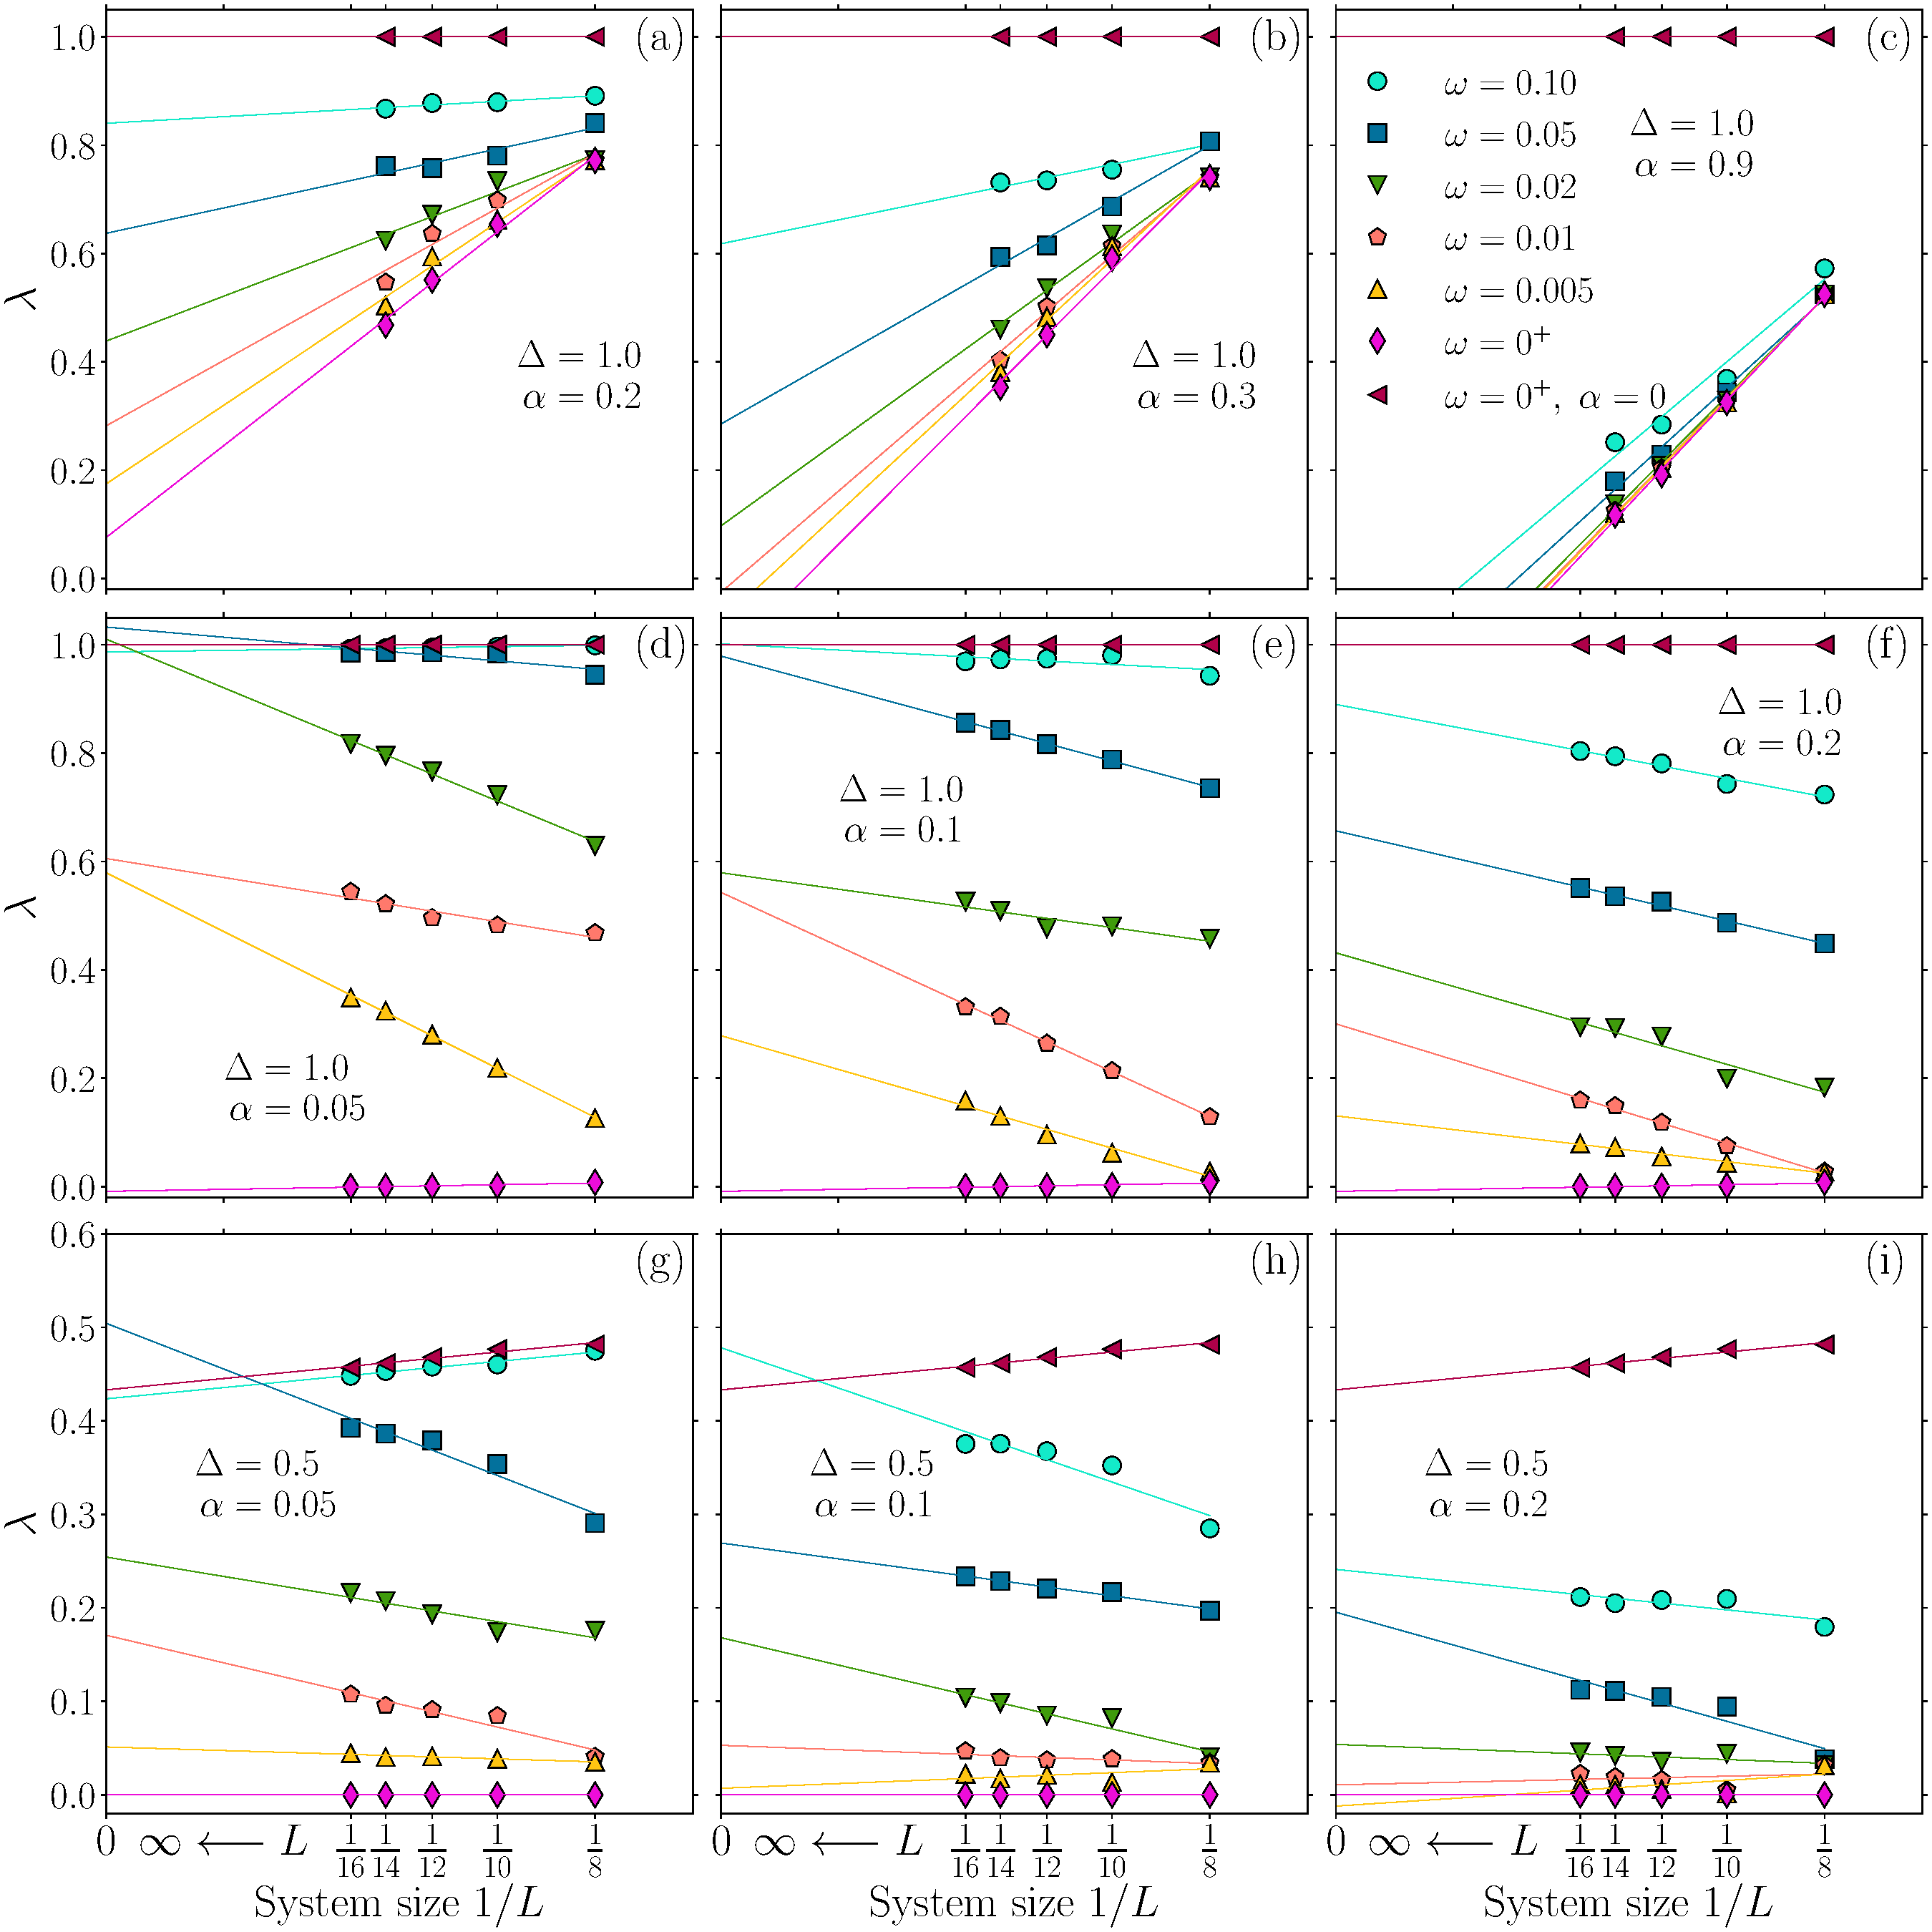
\includegraphics[width=\textwidth]{Figures/lioms_decay.pdf}
  \caption{Finite-time stiffness operators as a function of time for the perturbed Hamiltonian.
  Panels (a)-(c) show results for \(J^E\), (d)-(f) for \(\hat{O}_1\) and (g)-(i) for \(\hat{O}_2\).
  See text for detailed description.}
  \label{fig:lioms decay}
\end{figure}


\section{Relaxation of known (Q)LIOMs}
% After establishing the range of perturbation strengths relevant to our problem, we can now
To investigate how our (Q)LIOMs decay with time, we will apply the formalism of spectral functions
described in Sections~\ref{sec:spectral function}.
Since we are interested in the low-\(\omega\) (long times) part of integrated spectral function
\(I(\omega)\), it is convenient to normalize it. Therefore, let us define the
following~\autocite{Mierzejewski2015Approx}:
\begin{equation}
  R_{\hat{A}}(\omega,\alpha) = \frac{I(\omega,\alpha)}{\lim_{\omega \to 0^{+}} I(\omega,\alpha=0)} = 
  \frac{\sum_{n,m}\theta\left(\omega -\abs{E_n-E_m}\right) \abs*{\matrixel{m}{\hat{A}}{n}}^2}
  {\sum_{\substack{n,m \\ E_n=E_m}} \abs*{\matrixel{m}{\hat{A}}{n}}^2}
  \label{eq:normalized integrated spectral function}
\end{equation}
This normalization of \(I(\omega)\) assures that  \(\lim_{\omega\to \infty} R_{\hat{A}}
(\omega,\alpha) = 1\). However at first we should establish a range of values of
parameter \(\alpha\) so its small enough that \(H'\) remains a perturbation but large enough
to be relevant for finite system sizes accessible numerically. As mentioned in previous section,
we are looking vanishing infinite-time stiffness in thermodynamic limit. Therefore, we will
take \(\alpha\) as small as possible so that  \(\lim_{\omega\to 0^{+}} R_{\hat{A}}
(\omega,\alpha) = 0\).

\subsection{Relaxation of energy current}
We begin with the case energy current \(J^E\) for \(\Delta = 1.0\), as derived in Section~\ref{sec:energy current}.
In the integrable parent model it is a conserved quantity, so we have the following:
\begin{equation*}
  \hs{J^E(t)}{J^E} = const \implies S(\omega) \propto \delta(\omega)
  \implies R_{J^E}(\omega,\alpha=0) = 1
\end{equation*}
After moving away from integrable regime, the autocorrelation function starts to decay,
so the \(\delta\)-peak broadens and \(R_{J^E}(\omega,\alpha=0)\) is no longer equal to one,
but approaches zero as time increases. We will look simultaneously at two different situations,
results for \(L=14\) and results extrapolated to thermodynamic limit from \(L=11,12,13,14\). 
Figure~\ref{fig:current decay no scaling} shows \(R_{J^E}(\alpha,\omega)\) as a
function of \(\omega\) for \(\alpha=0.3,0.4,0.5\). We immediately see the expected outcome, as the
stronger the perturbation the faster the current decays. The fact that for finite \(L\),
\(R_{J^E}(\alpha,\omega)\) does not approach \(0\) in \(\omega\to 0^+\) limit is consistent
with results in Figure~\ref{fig:lioms decay}.
\begin{figure}[htbp]
  \centering
  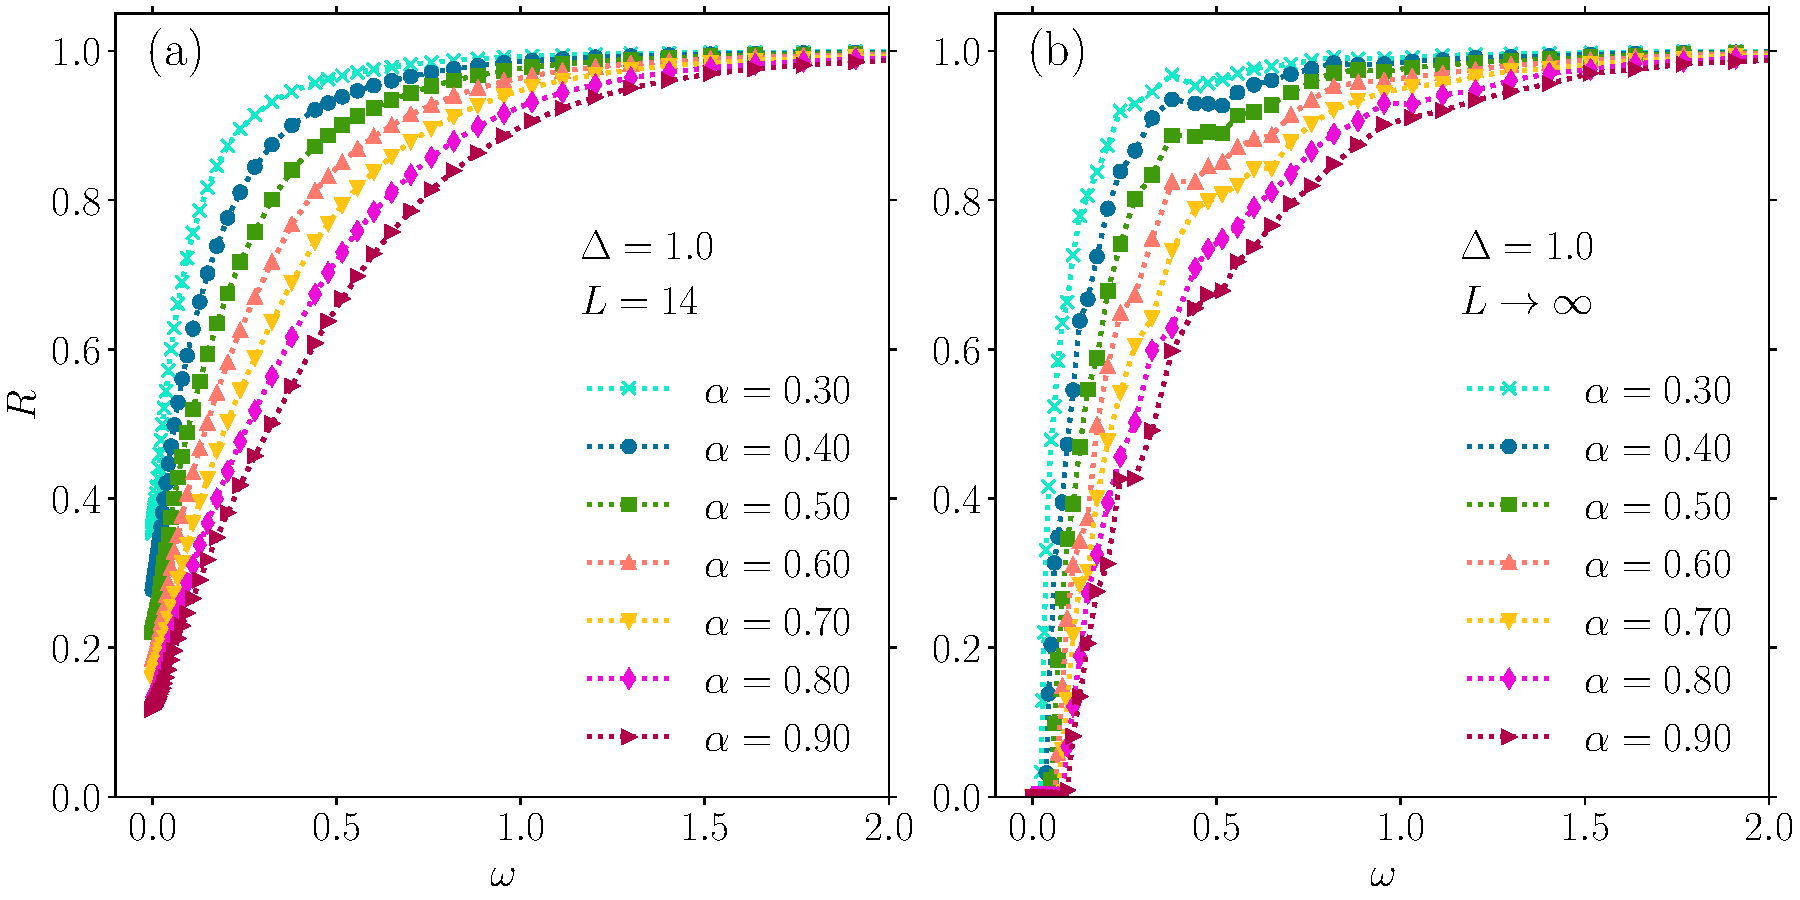
\includegraphics[width=\textwidth]{Figures/current_no_scaling.pdf}
  \caption{Normalized integrated spectral function as a function of cutoff frequency for \(J^E\).
  (a) Results for \(L=14\). Low frequency limit does not approach 0
  because of finite size effects. (b) Results extrapolated to thermodynamic limit from \(L=11,12,13,14\).
  Note the expected observation, namely stronger perturbation leads to faster decay.}
  \label{fig:current decay no scaling}
\end{figure}
\begin{figure}[htbp]
  \centering
  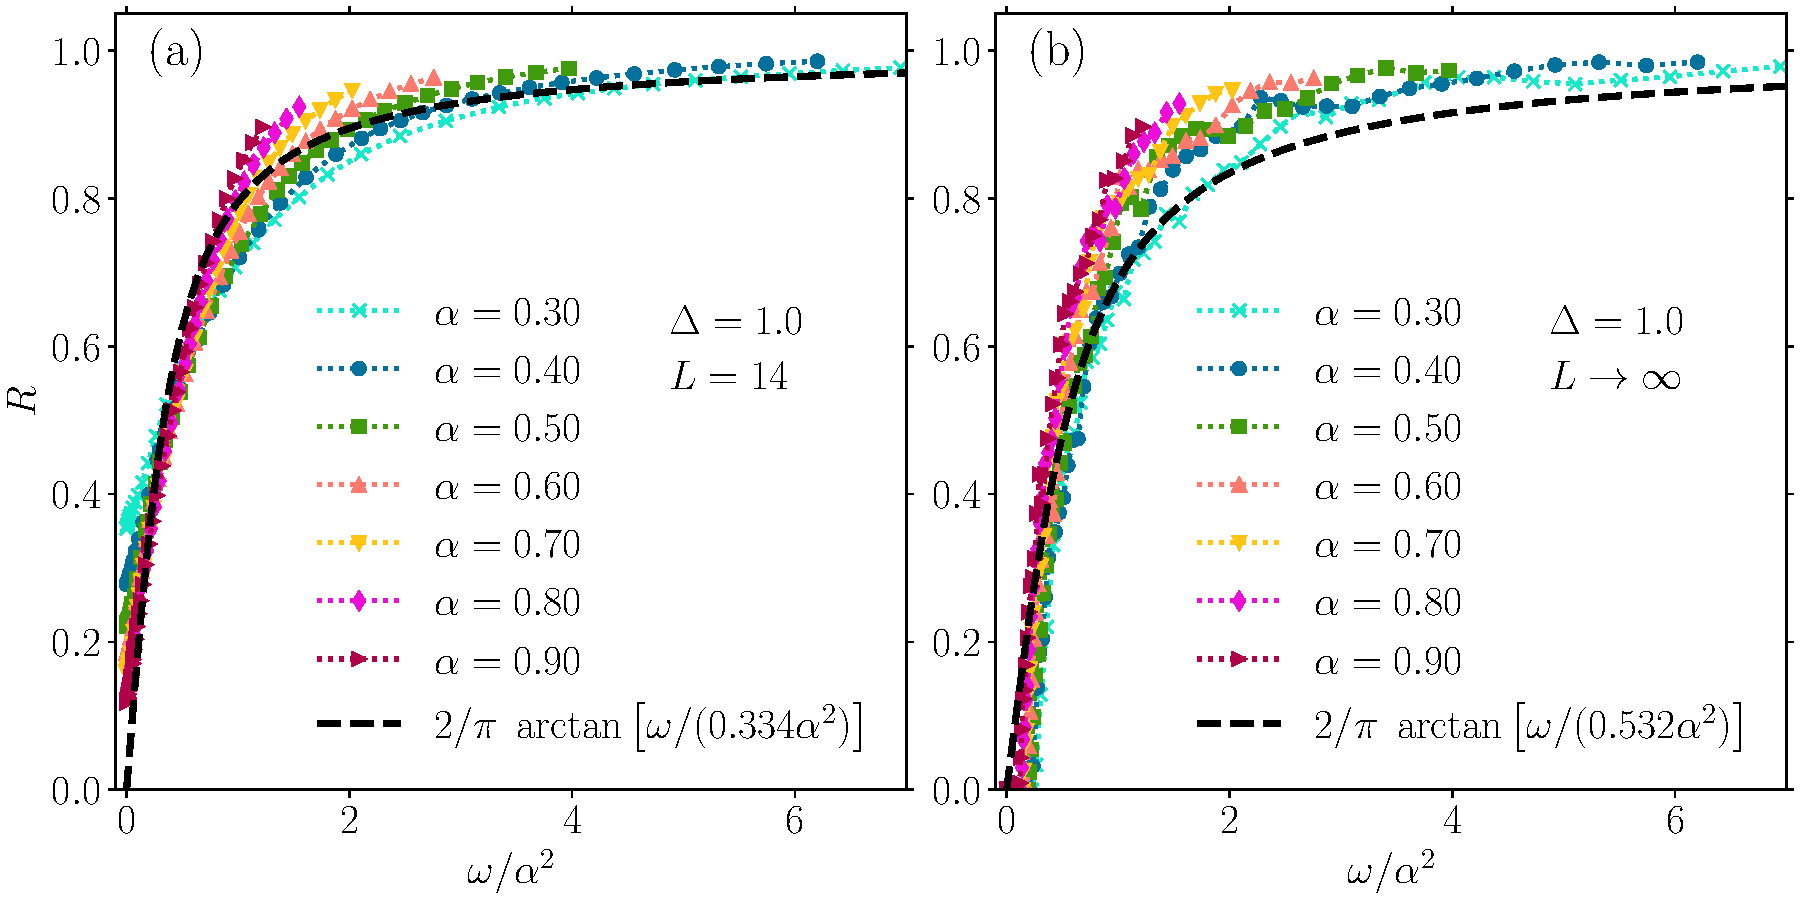
\includegraphics[width=\textwidth]{Figures/current_scaling.pdf}
  \caption{Normalized integrated spectral function as a function of rescaled cutoff frequency for \(J^E\).
  (a) Results for \(L=14\). (b) Results extrapolated to thermodynamic limit from \(L=11,12,13,14\).
  Dashed black line corresponds to fit~\eqref{eq:R arctan}.}
  \label{fig:current decay scaling}
\end{figure}
However, an interesting thing happens when plot the same data, but as a function of rescaled
frequency \(\omega/\alpha^2\). Numerical results visible on Figure~\ref{fig:current decay scaling}
show a convincing collapse of curves for different values of perturbation strength. This may suggest
an universal dependence of \(R(\omega,\alpha)\) on \(\omega\) and \(\alpha\):
\begin{equation}
  R(\omega,\alpha)\simeq \tilde{R}(\omega/\alpha^2)
  \label{eq:universal scaling current}
\end{equation}
Moreover, this relation can be reasonably well approximation by a one parameter fit
(black dashed line in Figure~\ref{fig:current decay scaling}):
\begin{equation}
  \tilde{R}(\omega/\alpha^2) \simeq \frac{2}{\pi} \arctan\left(\frac{\omega}{\gamma \alpha^2}\right)
\label{eq:R arctan}
\end{equation}
where \(\gamma \) is the fitting parameter. It implies that the relaxation of energy current
is exponential in nature. To see this, let us calculate \(I(\omega)\) for such decay
\(\hs{J^E(t)}{J^E} \propto e^{-\abs{t}/\tau_{J}}\). Double-sided exponential has well defined Fourier
transform, so we can drop the \(\epsilon \to 0^{+}\) limit from the integral.
\begin{align}
  S(\omega) &\propto \frac{1}{2\pi} \int_{-\infty}^{\infty} \mathrm{d} t\; e^{-\abs{t}/\tau_{J}} e^{i \omega t} = 
  \frac{1}{2\pi} \left[\int_{-\infty}^{0} \mathrm{d} t\; e^{(1/\tau_{J} + i\omega)t }
  + \int_{0}^{\infty} \mathrm{d} t\; e^{(-1/\tau_{J} + i\omega)t }  \right] \nonumber \\
  &= \frac{1}{2\pi} \left[\frac{\tau_{J}}{1+i\omega \tau_{J}} + \frac{\tau_{J}}{1-i\omega\tau_{J}}\right] = 
  \frac{1}{\pi} \frac{\tau_{J}}{1+\omega^2\tau_{J}^2}
\end{align}
Integrating \(S(\omega)\) over a frequency window we obtain:
\begin{equation*}
  I(\omega) \propto \frac{1}{\pi}\int_{-\omega}^{\omega}\mathrm{d}\omega^{\prime}\; 
  \frac{\tau_{J}}{1+\omega^2\tau_{J}^2} = \frac{2}{\pi} \arctan(\tau_{J} \omega)
\end{equation*}
which after normalization yields the desired results~\eqref{eq:R arctan}. Furthermore, we learn that the 
characteristic relaxation time \(\frac{1}{\tau_{J}} \propto \alpha^2\) and the proportionality
constant is universal and does not depend on \(\alpha\).
The quadratic scaling shown on Figure~\ref{fig:current decay scaling} is actually not the
best possible for this set of numerical data. Choosing the rescaling coefficient to be
\(\frac{3}{2}\) allows for almost perfect collapse of all the curves 
(see Figure~\ref{fig:current decay perfect scaling}). However, it is expected to be a consequence
of working with rather small system sizes, because in was shown 
in~\textcite{Mierzejewski2015Approx} using memory function formalism, that quadratic scaling
is indeed the appropriate one.
\begin{figure}[htbp]
  \centering
  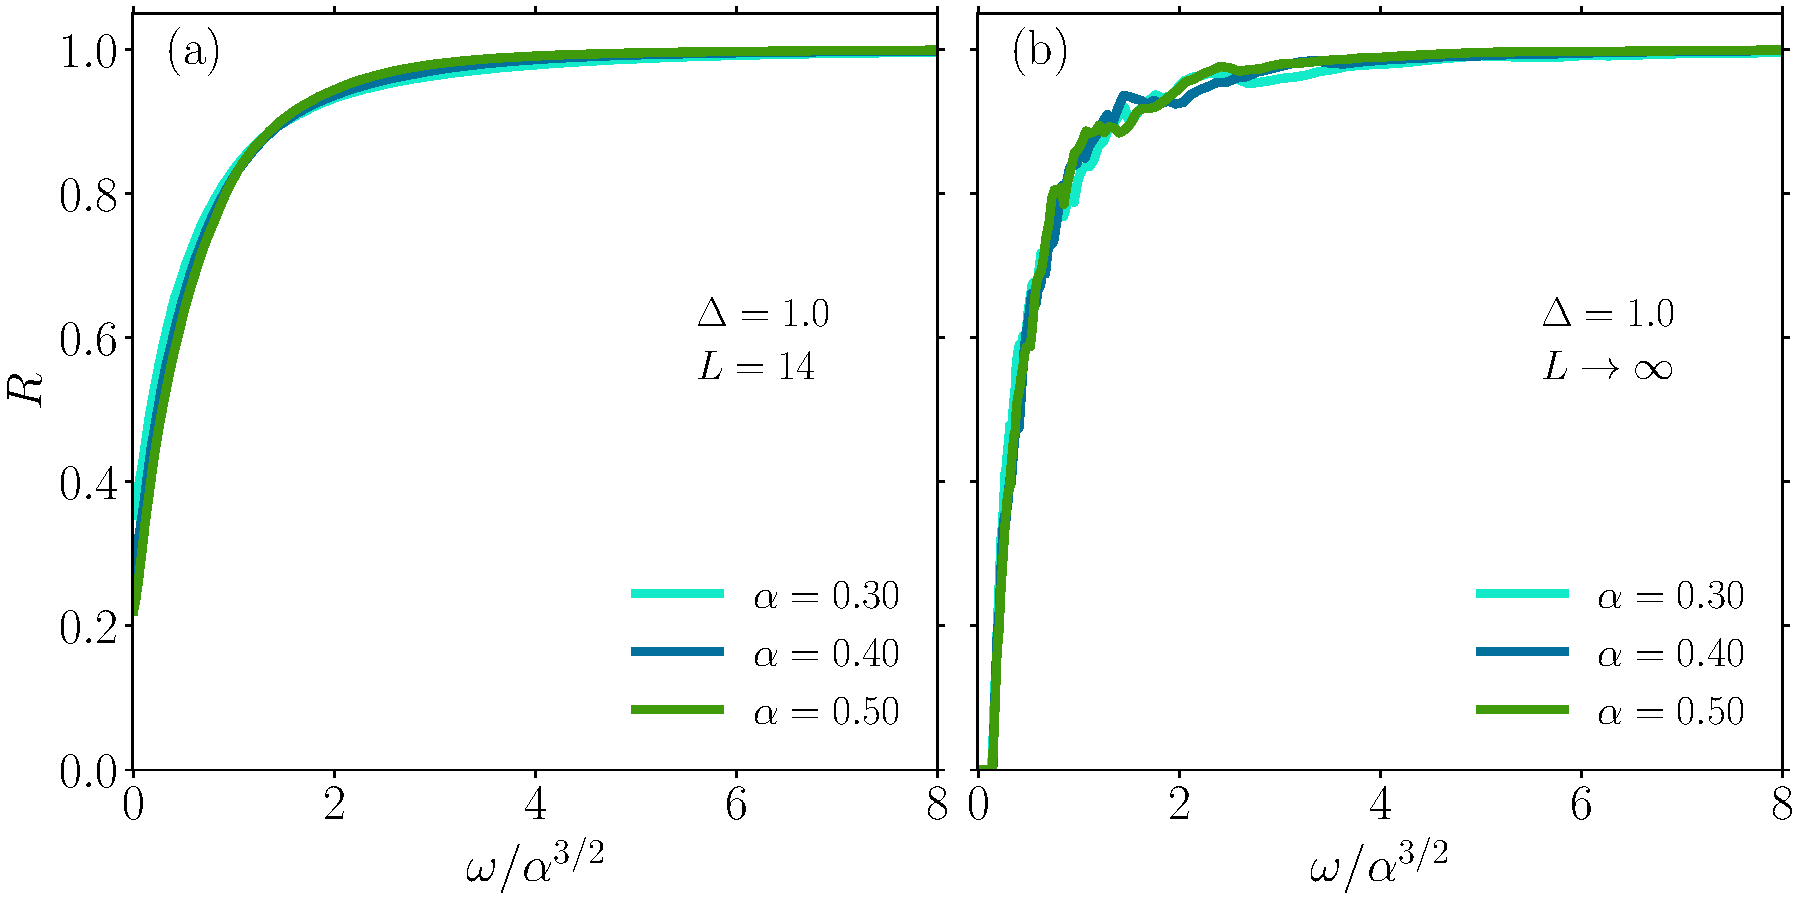
\includegraphics[width=1.0\textwidth]{Figures/current_perfect_scaling.pdf}
  \caption{Normalized integrated spectral function as a function of 
  rescaled cutoff frequency for \(J^E\). The rescaling coefficient is chosen so as to obtain the 
  best possible collapse of curves. (a) Results for \(L=14\). (b) Results extrapolated
   to thermodynamic limit from \(L=11,12,13,14\).}\label{fig:current decay perfect scaling}
\end{figure}


\subsection{Relaxation of noncommuting (Q)LIOMs}
Let us now proceed with the same analysis, but for the \(\hat{O}_1\)~\eqref{eq:delta 1.0} 
and \(\hat{O}_2\)~\eqref{eq:delta 0.5} operators. Once again we shall look at the largest
system size available to us, that is \(L = 16\), as well as the case of extrapolation
to thermodynamic limit from \(L = 10,12,14,16\). 
Figure~\ref{fig:O12 no scaling} shows
\(R_{\mu}(\omega,\alpha)\), where \(\mu=1,2\), as a function of \(\omega\) for \(\alpha = 0.05,0.1,0.2\).
We have used weaker perturbations here, because Figure~\ref{fig:lioms decay} suggested that
it is enough to achieve vanishing stiffness in thermodynamic limit. Indeed this is the case
and we observe that \(\lim_{{\omega\to 0^{+}}} R_{\mu}(\omega,\alpha) = 0\) even for finite-size systems.
Basing on the discussion of energy current decay, next logical step would be to rescale the
frequency by \(\alpha^2\).

\begin{figure}[htbp]
  \centering
  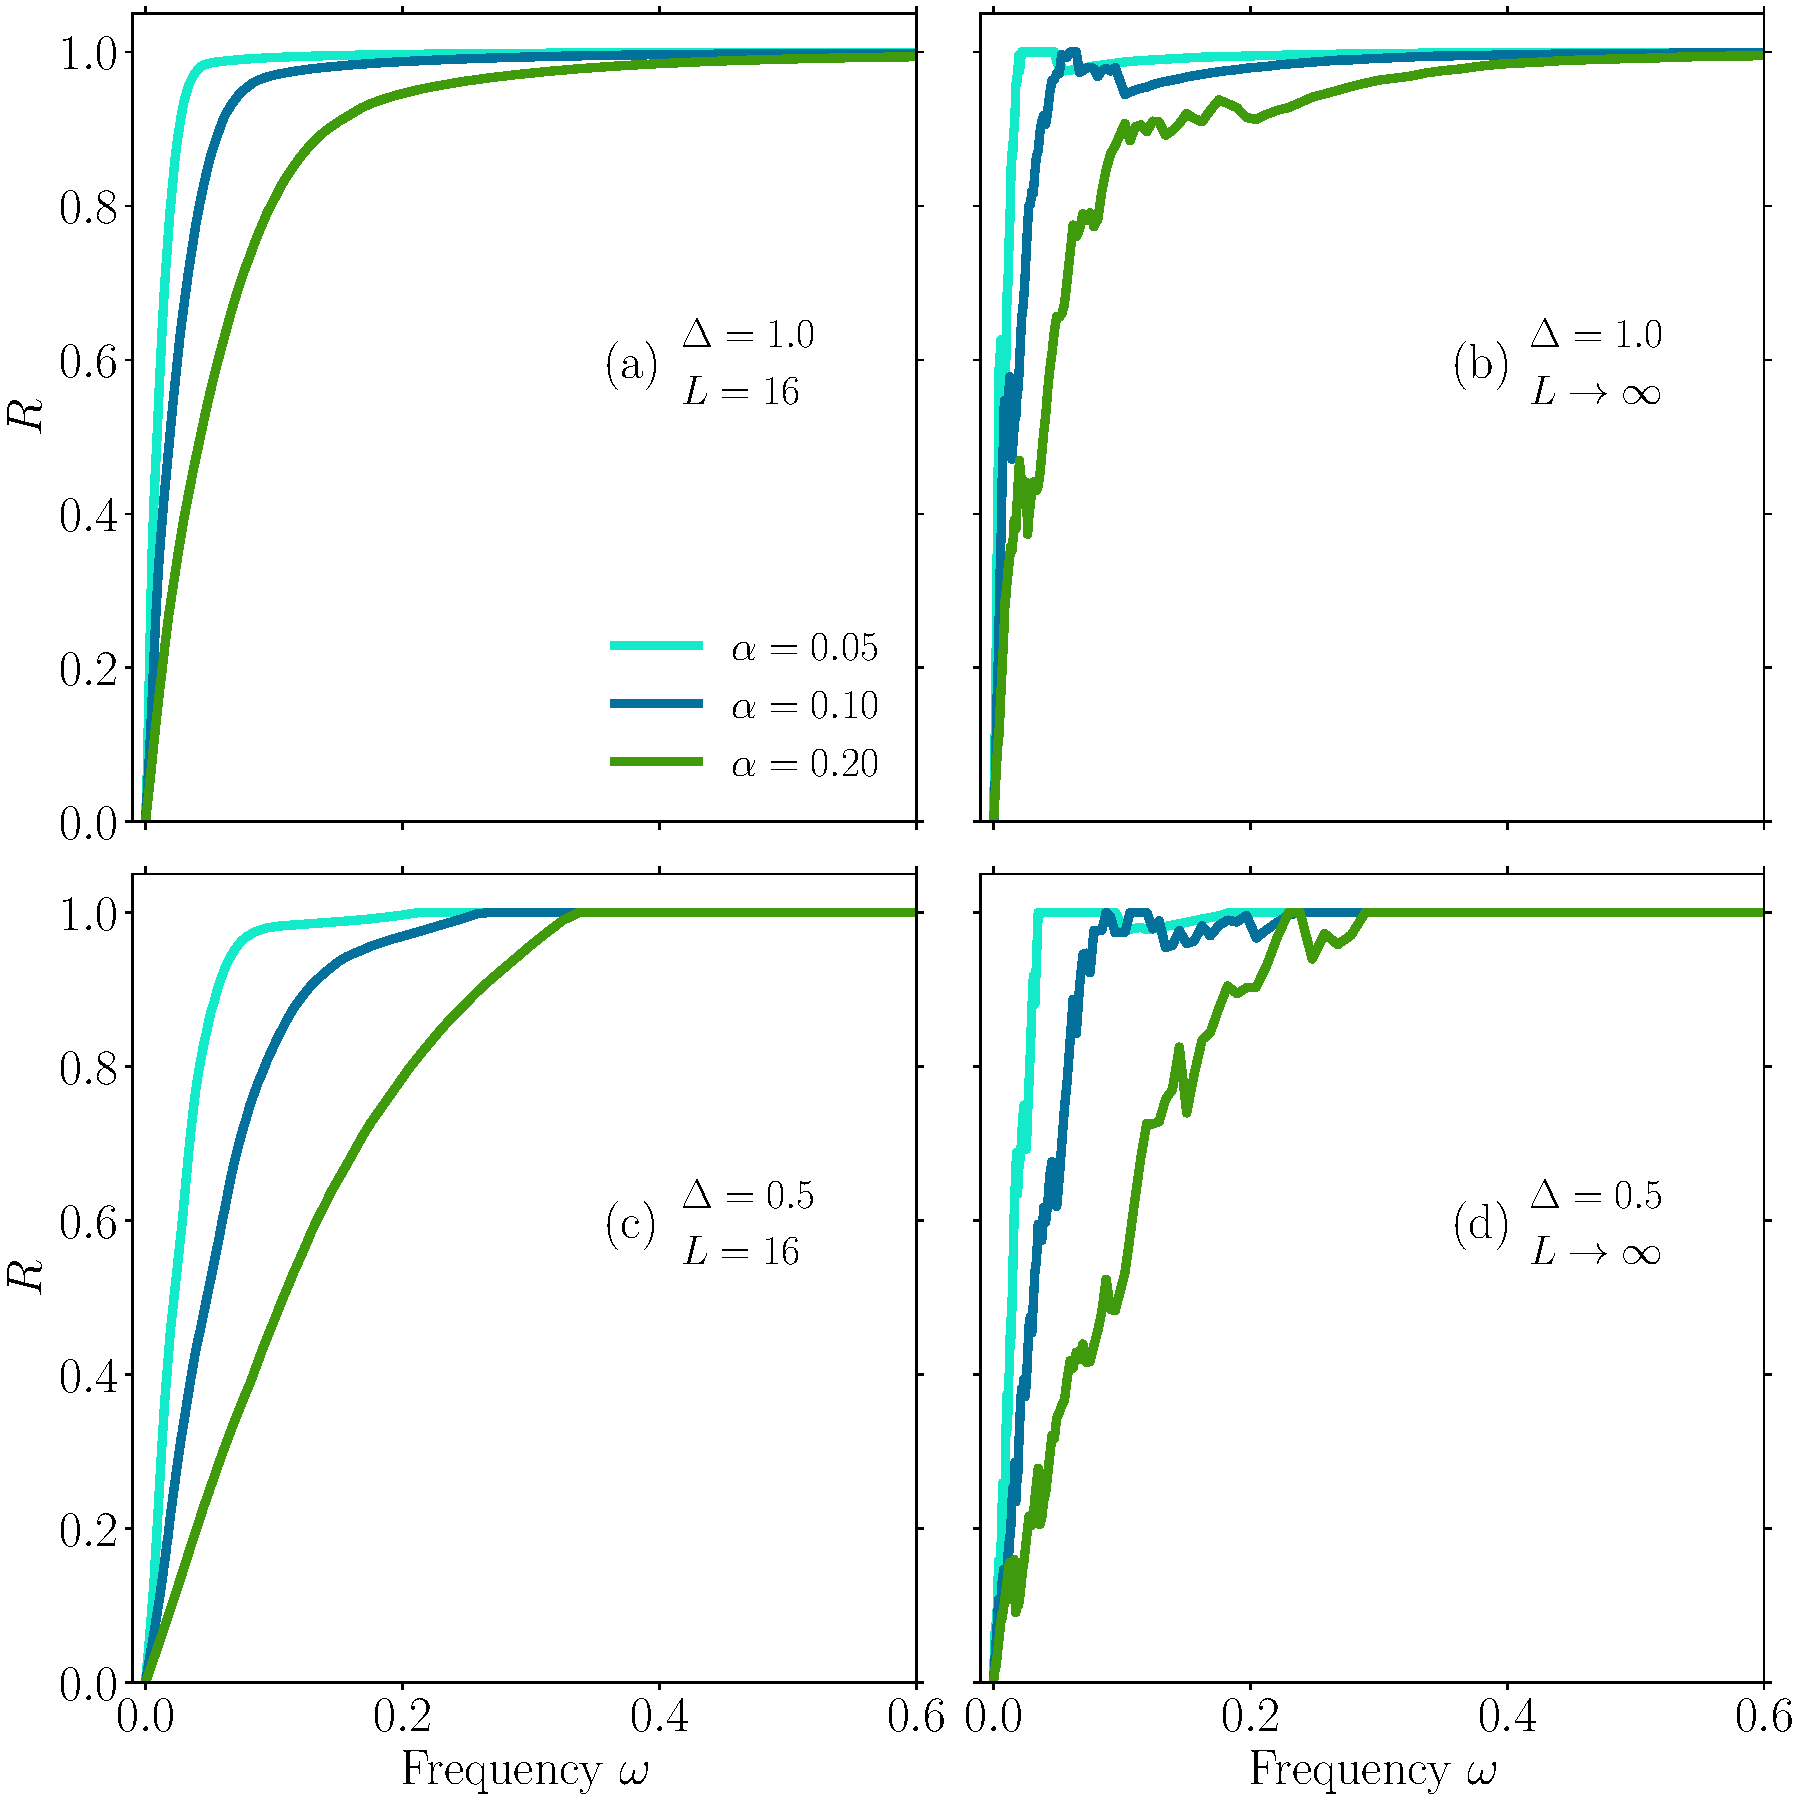
\includegraphics[width=1.0\textwidth]{Figures/O12_no_scaling.pdf}
  \caption{Normalized integrated spectral function as a function of cutoff frequency for
  \(\hat{O}_1\) and \(\hat{O}_2\).
  (a) Results for \(L=16\) and \(\hat{O}_1\).  (b) Results for \(\hat{O}_1\) extrapolated to
  thermodynamic limit from \(L=10,12,14,16\). (c) Results for \(L=16\) and \(\hat{O}_2\). 
  (d) Results for \(\hat{O}_2\) extrapolated to thermodynamic limit from \(L=10,12,14,16\).
  Note that low frequency limit for finite system does approach \(0\), as expected from 
  Figure~\ref{fig:lioms decay}.
  }\label{fig:O12 no scaling}
\end{figure}

In contrast to the energy current, we not see any collapse (see Figure~\ref{fig:O12 quadratic scaling}).
Therefore, noncommuting operators do not follow the same universal scaling~\eqref{eq:universal scaling current}
as the energy current. However, as shown in Figure~\ref{fig:O12 linear scaling},
it turns out that a reasonable collapse, working for both \(\hat{O}_1\) and \(\hat{O}_2\),
may be observed for a different scaling, namely \(\omega/\alpha\). This suggests another kind
of relation:
\begin{equation}
  R_{\mu}(\omega,\alpha) \simeq \tilde{R}_{\mu}(\omega/\alpha)
\end{equation}
Moreover, the collapsed curves can be accurately fitted with an one-parameter error function
 (black dashed line in Figure~\ref{fig:O12 linear scaling}):
\begin{equation}
  \tilde{R}_{\mu}(\omega/\alpha) \simeq \erf\left(\frac{\omega}{\gamma \alpha}\right)
  \label{eq:erf fit}
\end{equation}
where the fitting parameter in denoted with \(\gamma\) and error function is defined as:
\begin{equation}
\erf(x) = \frac{2}{\sqrt{\pi}} \int_{0}^{x} \mathrm{d}t\; e^{-t^2}  
\end{equation}
This implies a Gaussian, instead of
exponential, decay of autocorrelation function, i.e.\ \(\hs{\hat{O}_{\mu}(t)}{\hat{O}_{\mu}}
\propto \exp(-(t/\tau_{\mu})^2)\). We can once again make use of integrated spectral function
to see that this is correct.
\begin{align}
  S(\omega) &\propto \frac{1}{2\pi} \int_{-\infty}^{\infty} \mathrm{d}t \; e^{-(t/\tau_{\mu})^2}
  e^{i\omega t} = \frac{1}{2\pi} \int_{-\infty}^{\infty} \mathrm{d}t \; 
  \exp\left(-\frac{1}{\tau_{\mu}^2} \left(t-\frac{i\omega\tau_{\mu}}{2}\right)^2 
  - \frac{\omega^2\tau_{\mu}^2}{4}\right) \nonumber \\
  &= \exp\left(- \frac{\omega^2\tau_{\mu}^2}{4}\right) \frac{1}{2\pi}
  \int_{-\infty+\frac{i\omega\tau_{\mu}}{2}}^{\infty+\frac{i\omega\tau_{\mu}}{2}} 
  \mathrm{d} z\; \exp\left(-\frac{z^2}{\tau_{\mu}^2}\right) \nonumber\\
  & \triangleq \exp\left(- \frac{\omega^2
  \tau_{\mu}^2}{4}\right) \frac{1}{2\pi} \int_{-\infty}^{\infty}
  \mathrm{d} z\; \exp\left(-\frac{z^2}{\tau_{\mu}^2}\right) \nonumber  \\
  &= \frac{\tau_{\mu}}{2\sqrt{\pi}}e^{-(\omega \tau_{\mu}/2)^2}
\end{align}
where between first and second line a change of variables \(z = t-\frac{i \omega \tau_{\mu}}{2}\)
has been made, and equality marked with \(\triangleq\) can be justified by means of contour
integration~\autocite{Stein2010}. Now we can easily perform integration over a finite
frequency window:
\begin{align}
  I(\omega) &\propto \frac{\tau_{\mu}}{2\sqrt{\pi}}\int_{-\omega}^{\omega} \mathrm{d}\omega^{\prime}\;
  e^{-(\omega/\tau_{\mu})^2} = \frac{\tau_{\mu}}{2\sqrt{\pi}}
  \left[\int_{-\omega}^{0} \mathrm{d}\omega^{\prime} e^{-(\omega\tau_{\mu}/2)^2} + 
  \int_{0}^{\omega} \mathrm{d}\omega^{\prime} e^{-(\omega\tau_{\mu}/2)^2} \right]\nonumber\\
  &= \frac{\tau_{\mu}}{2\sqrt{\pi}} \left[ \frac{2}{\tau_{\mu}}\int_{-\frac{\omega\tau_{\mu}}{2}}^{0} 
  \mathrm{d} x\;  e^{-x^2} + \frac{2}{\tau_{\mu}}\int_{0}^{\frac{\omega\tau_{\mu}}{2}}
   \mathrm{d}x\; e^{-x^2} \right]\nonumber\\ 
   &= \frac{1}{\sqrt{\pi}} \left[ \frac{\sqrt{\pi}}{2} \erf\left(\frac{\omega\tau_{\mu}}{2}\right) +
   \frac{\sqrt{\pi}}{2} \erf\left(\frac{\omega\tau_{\mu}}{2}\right) \right]\nonumber\\
    &= \erf\left(\frac{\omega\tau_{\mu}}{2}\right)
\end{align}
where between first and second lines a change of variables \(x=\omega\tau_{\mu}/2\) has been made.
We have thus obtained the desired result~\ref{eq:erf fit}. On the contrary to the case of energy
current, the scaling of decay rate is \(\frac{1}{\tau_{\mu}} \propto \alpha\). This Gaussian relaxation
of noncommuting integrals of motion under weak perturbation is the main finding of this work.
\begin{figure}[htbp]
  \centering
  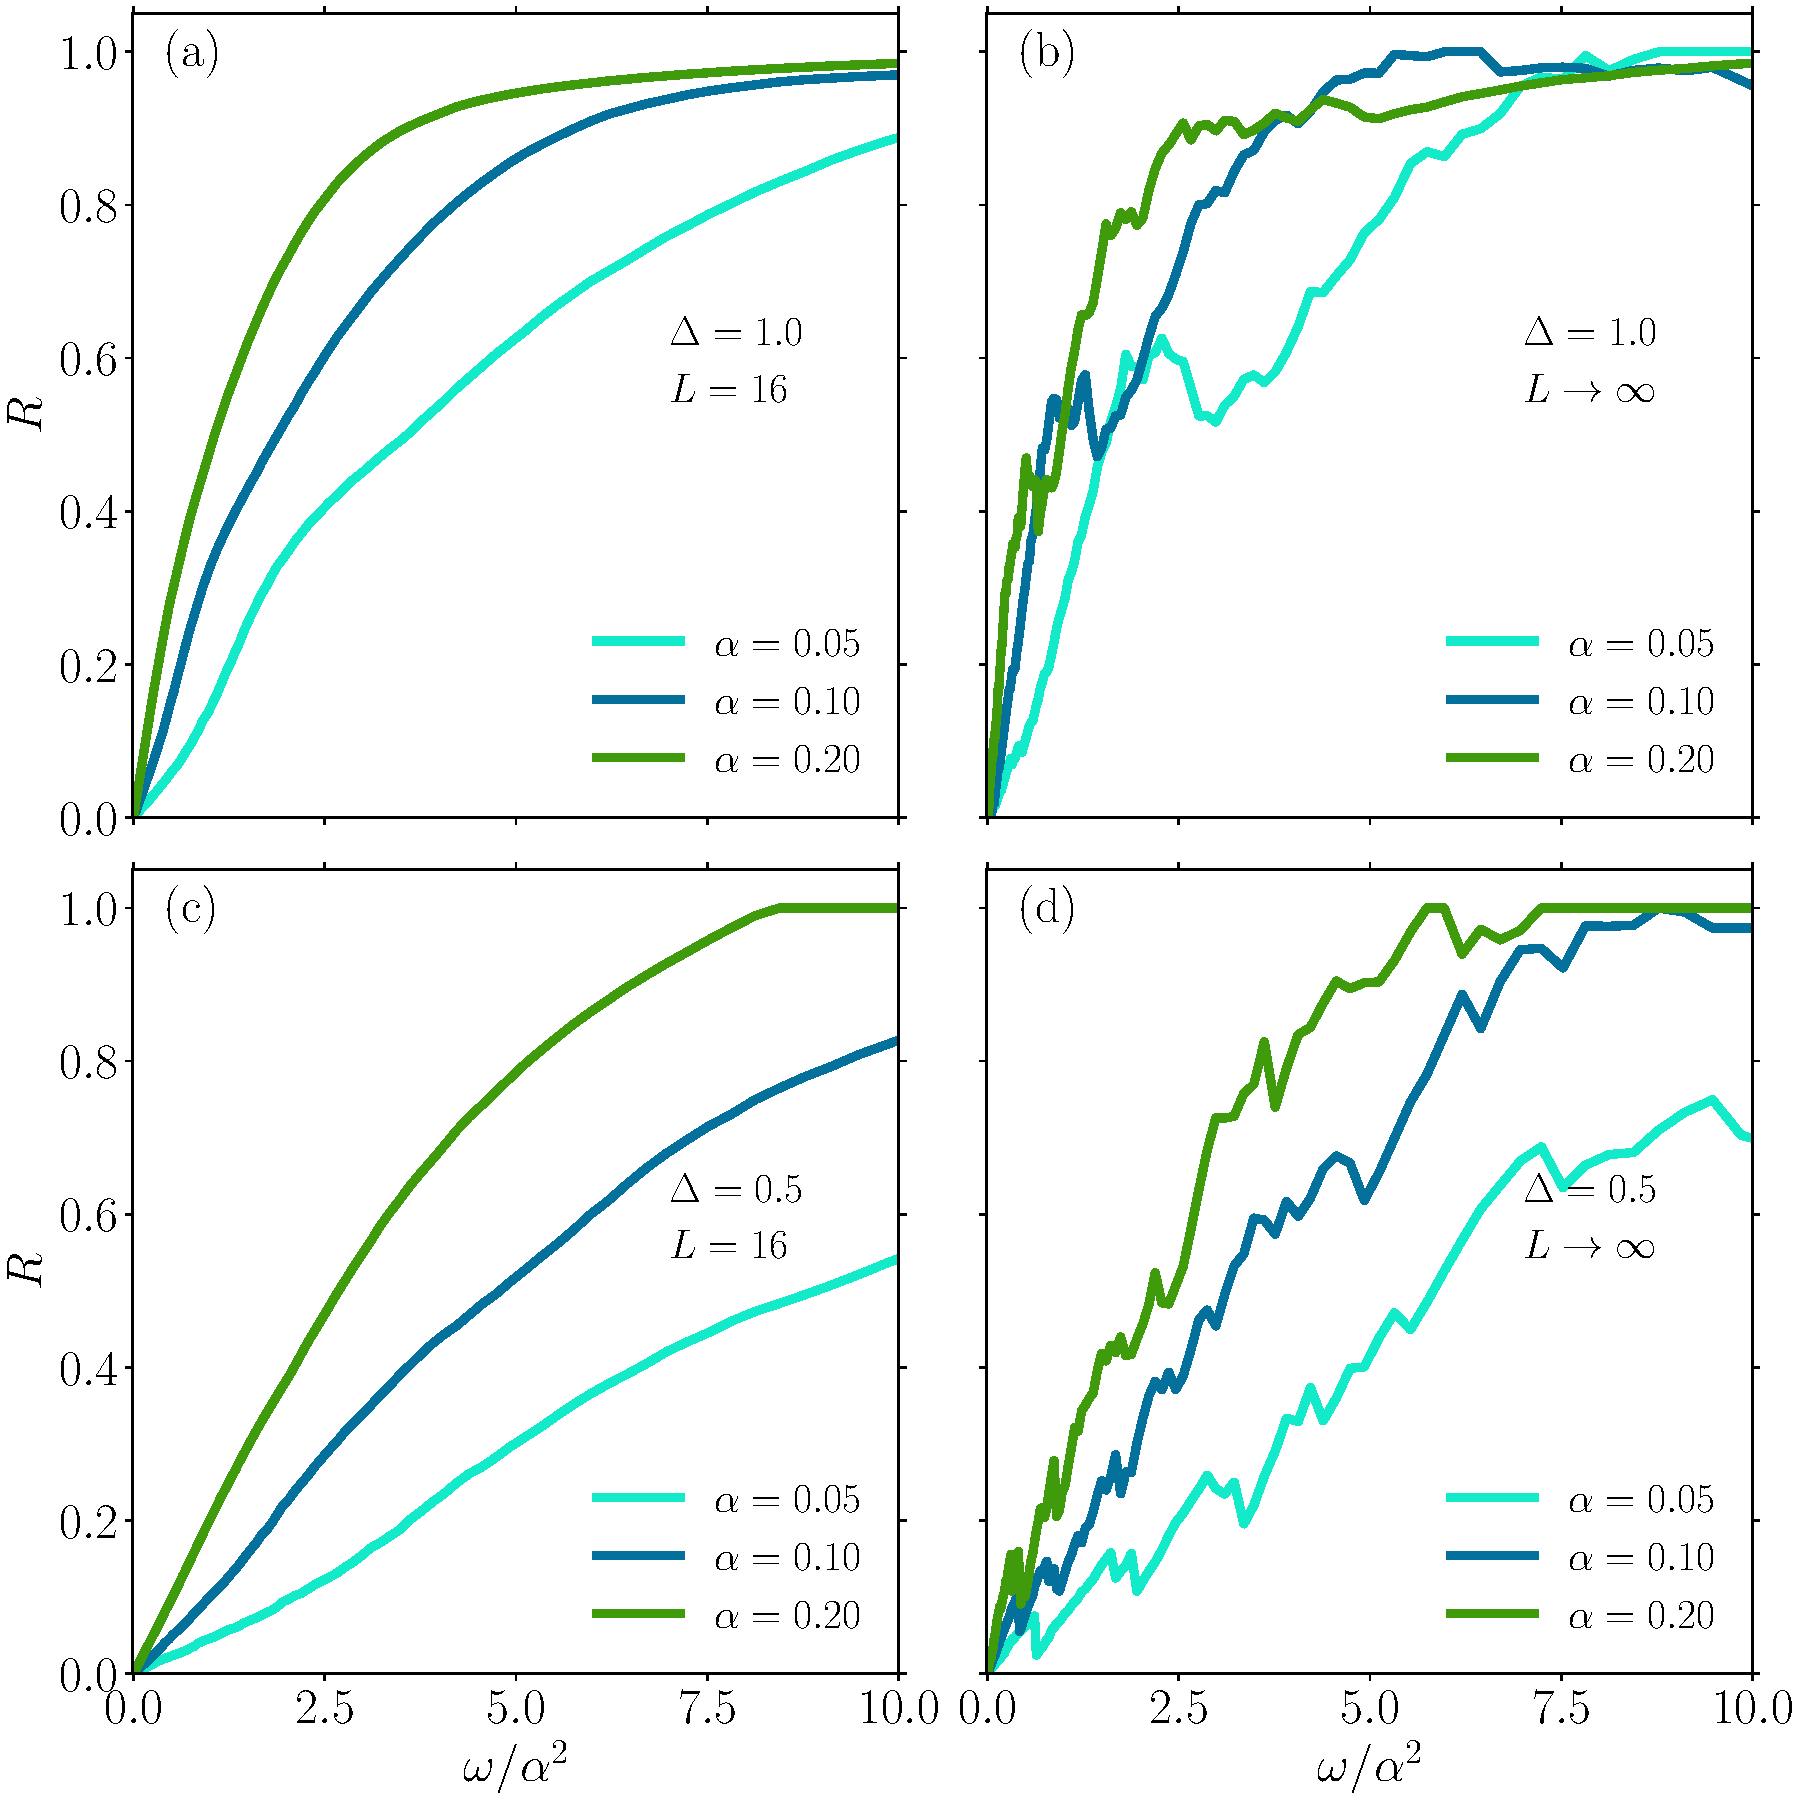
\includegraphics[width=1.0\textwidth]{Figures/O12_quadratic_scaling.pdf}
  \caption{}\label{fig:O12 quadratic scaling}
\end{figure}
\begin{figure}[htbp]
  \centering
  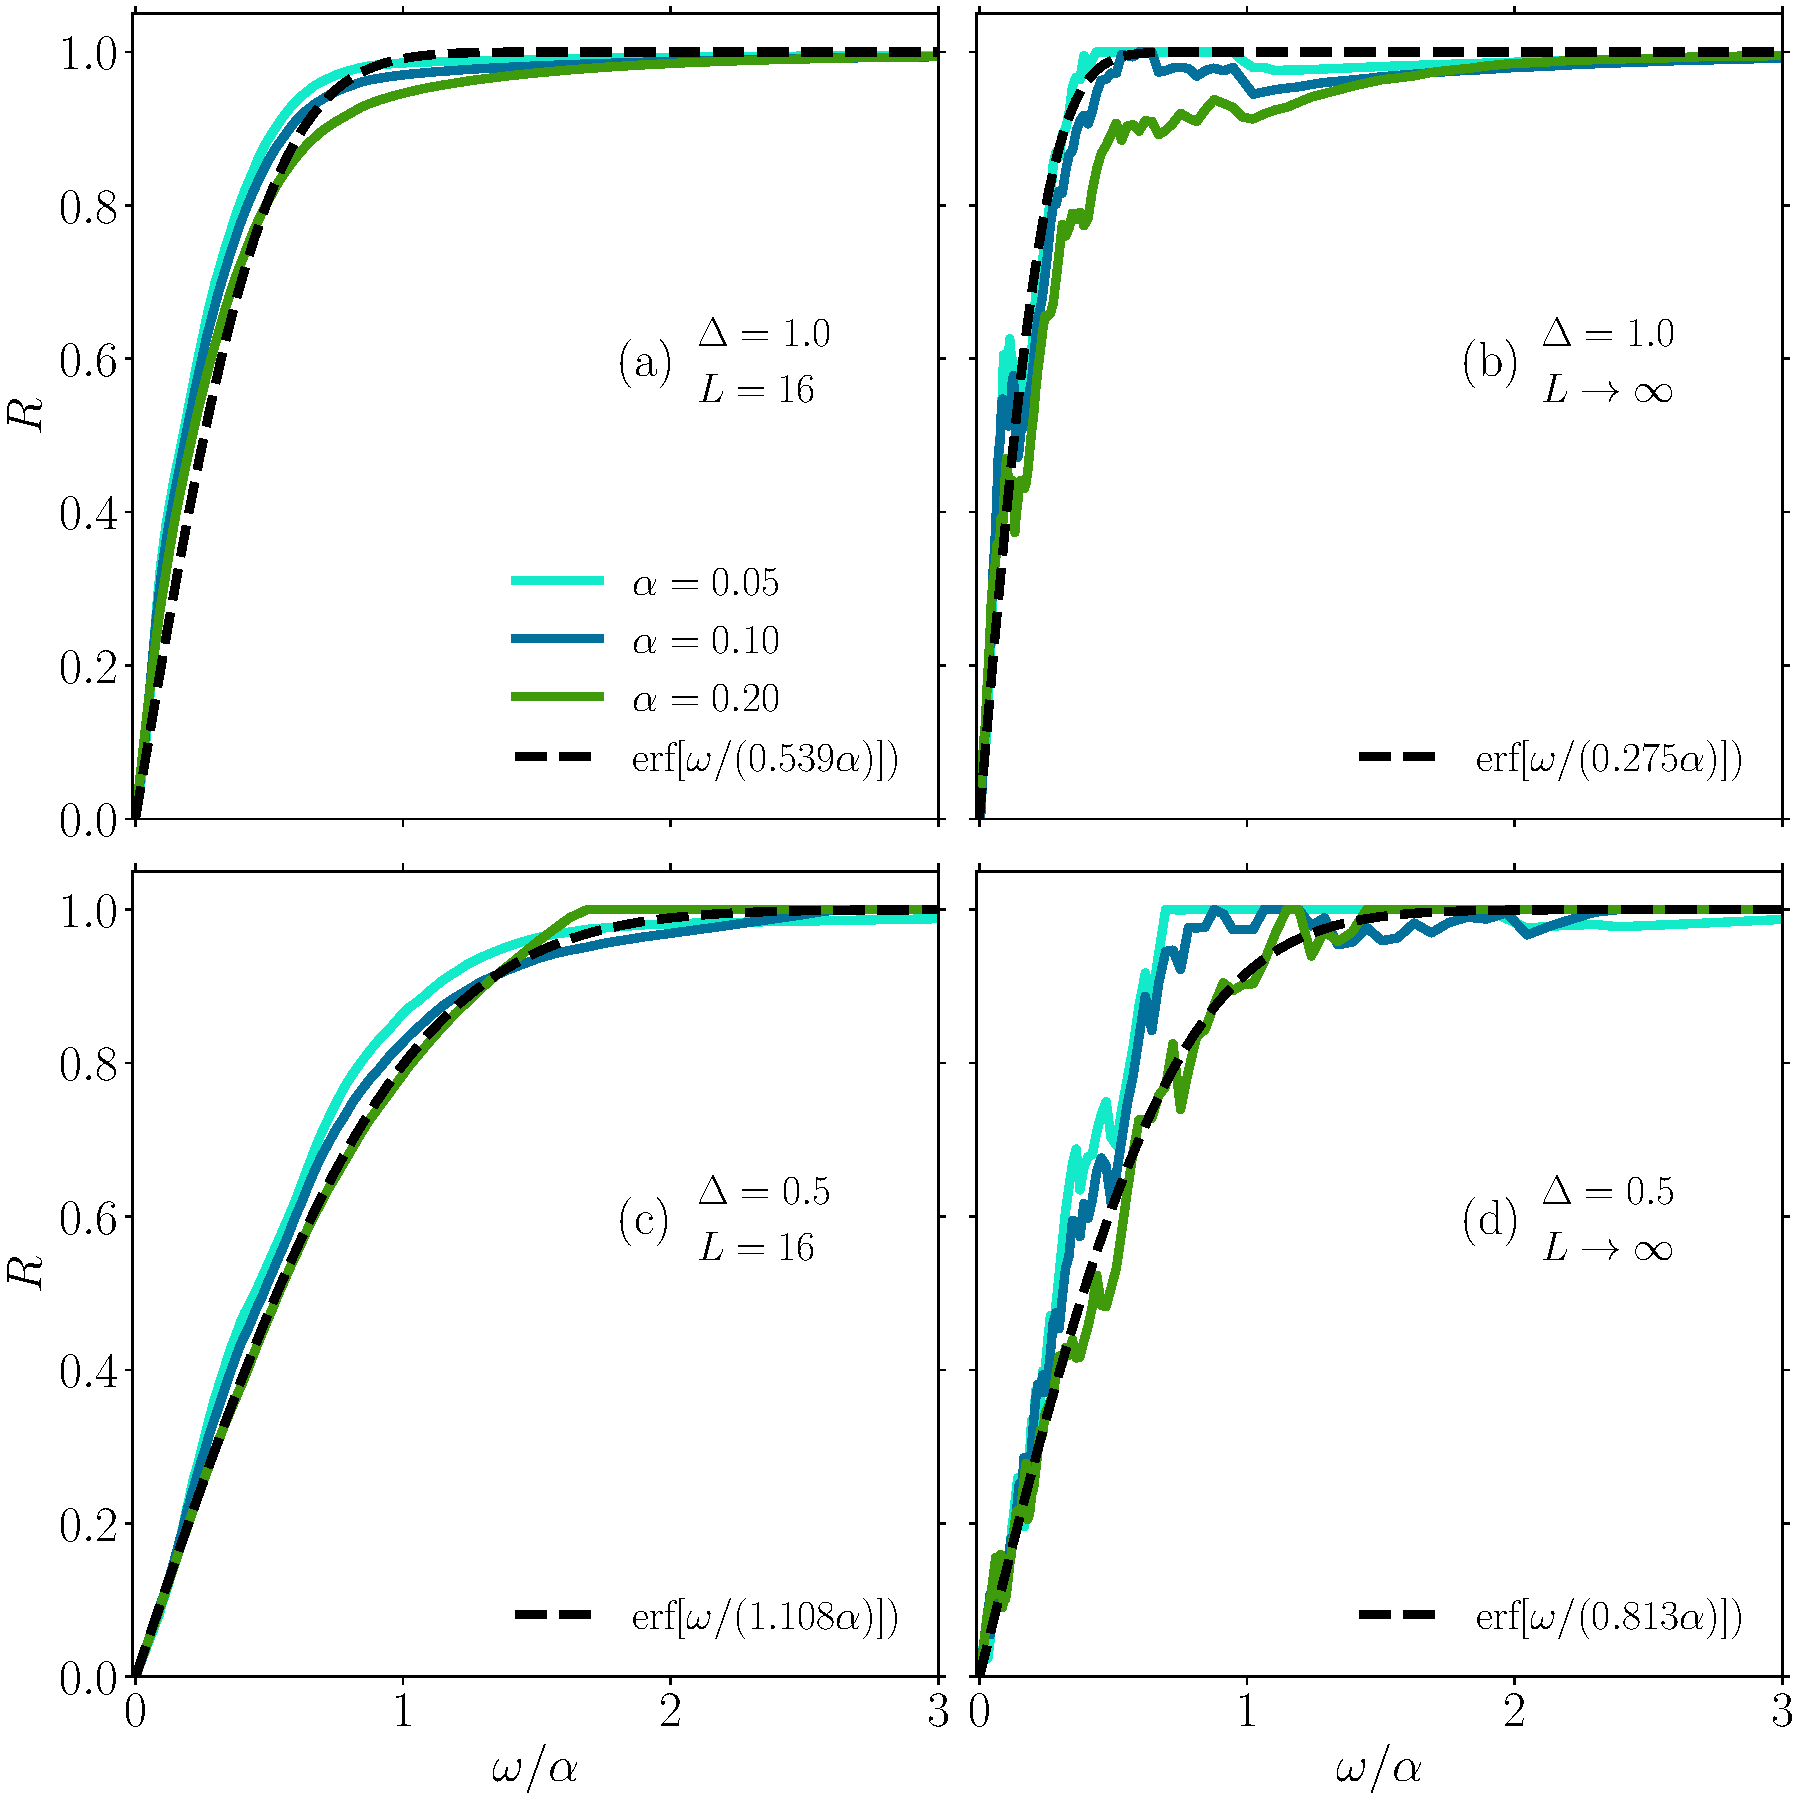
\includegraphics[width=1.0\textwidth]{Figures/O12_linear_scaling.pdf}
  \caption{}\label{fig:O12 linear scaling}
\end{figure}

One may ask a question about the origin of this anomalous scaling of characteristic time
\(\tau\). As noted in Subsection~\ref{subsec:noncomm qlioms}, operators exhibiting such scaling
are closely related to the massive degeneracies in energy spectrum of \(H_{XXZ}\) for
anisotropy  \(\Delta=1.0\) and \(\Delta = 0.5\), which is caused by states with
different total magnetization \(\Sz_{tot}\) but
equal energies. This in turn, is caused by certain symmetries of the Hamiltonian, simple \(SU(2)\) for
the former case and much more complex \(U_q(\mathfrak{sl}_2)\) for the latter 
case~\footnote{Technically, this symmetry is present only for \(\Delta=-0.5\), but this
can be amended in thermodynamic limit for chains of even length, as discussed in 
Subsection~\ref{subsec:noncomm qlioms}. }. 
When adding perturbation~\eqref{eq:perturbation}, there are actually two mechanism at play. We break
integrability while simultaneously breaking symmetry and thus lifting the macroscopic degeneracy.
We can disentangle these two mechanism, by studying behavior of \(\hat{O}_1\) and \(\hat{O}_2\)
under a different perturbation, namely:
\begin{equation}
  H^{\prime\prime} = \delta \sum_{j=1}^{L} \Sz_j \Sz_{j+1}
\end{equation}
This is equivalent to the unperturbed Hamiltonian for \(\Delta^{\prime} = \Delta + \delta\),
and allows us to eliminate degeneracy while preserving integrability. Results of this procedure
are shown in Figure~\eqref{eq:O12 symmetry}. We see almost the same behavior as for system
with weakly broken integrability, i.e.\ the relaxation is Gaussian in nature with the
characteristic decay rate inversly proportional to \(\delta\). It is not the lack of
integrability but lack of symmetry-related degeneracy, occurring for either \(\alpha\neq 0\)
or \(\delta\neq 0\), that leads to this anomalous scaling.

\textcolor{blue}{what about first-order perturbation theory?}
\begin{figure}[htbp]
  \centering
  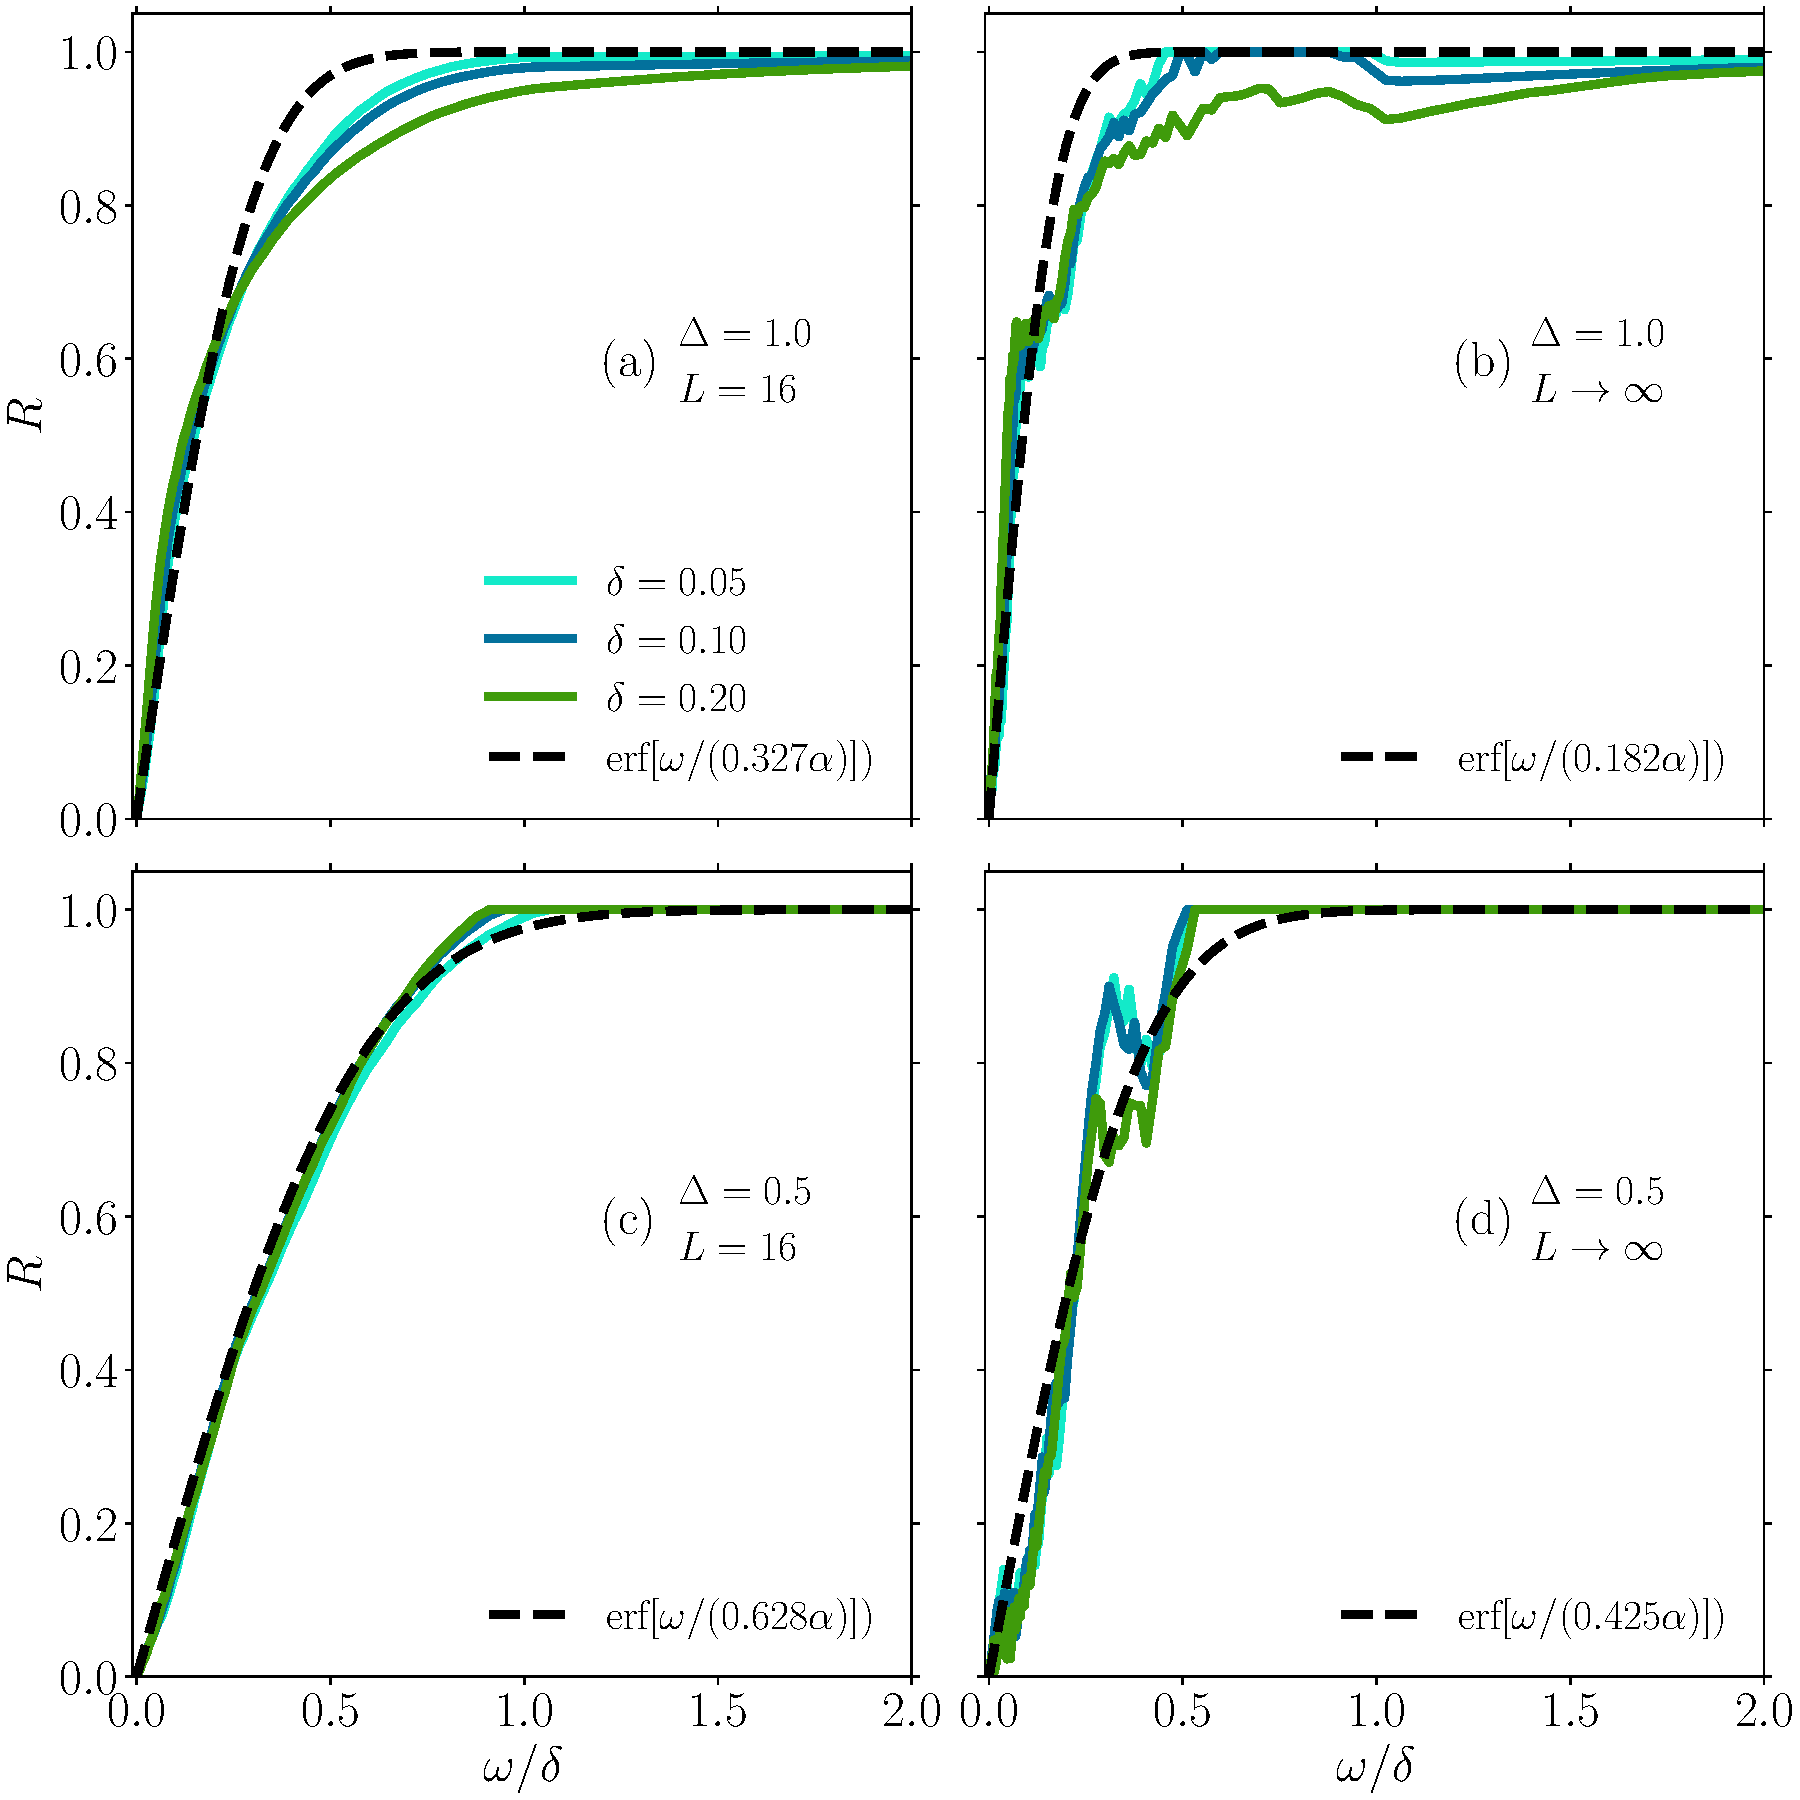
\includegraphics[width=1.0\textwidth]{Figures/O12_symmetry_breaking.pdf}
  \caption{}\label{fig:O12 symmetry}
\end{figure}

	\cleardoublepage{}

	\chapter{scratchpad}
\thispagestyle{chapterBeginStyle}

In this work we will describe \ldots~\autocite{Mierzejewski2015a}



\noindent Quantity that is plotted in Figures~4--14:
\begin{itemize}
    \item 
    With extrapolation to thermodynamic limit:
    \begin{equation}
        R_l(\tau,\alpha) = \frac{\lambda_l(L\rightarrow \infty,\tau,\alpha)}
        {\lambda_l(L\rightarrow \infty,\tau \rightarrow \infty,\alpha=0)}
        \label{eq:R1 extrap}
    \end{equation}
    \item
    Without extrapolation to thermodynamic limit:
    \begin{equation}
        R^L_l(\tau,\alpha) = \frac{\lambda_l(L,\tau,\alpha)}
        {\lambda_l(L,\tau \rightarrow \infty,\alpha=0)}
        \label{eq:R1 no extrap}
    \end{equation}
\end{itemize}


\noindent Energy current in integrable XXZ model: 
\begin{align}
    J^E = \sum_i^L i\left[\beta_1 \left(\Sm_{i-1}\Sz_{i}\Sp_{i+1}\right) + \beta_2 \left(\Sz_{i-1}\Sp_{i}\Sm_{i+1}+\Sp_{i-1}\Sm_{i}\Sz_{i+1}\right)\right] + \text{H.c.}
\end{align}


\noindent Spin LIOM for \(\Delta=1.0\):
\begin{equation}
    \hat{O}_{1} =  \beta_3\sum_{i=1}^{L} \Sp_{i} + \text{H.c.}
\end{equation}

\noindent Spin QLIOM for \(\Delta=-0.5\):
\begin{equation}
    \hat{O}_{1} =\beta_4 \sum_{i=1}^{L} \Bigl( \Sp_{i}\Sp_{i+1}\Sp_{i+2}\Bigr) + \text{H.c.}
\end{equation}

\begin{equation*}
    \comm{J^E}{\Sz_{tot}} = 0 \text{   where   } \Sz_{tot} = \sum_i \Sz_i
  \end{equation*}
  
  
\section{Operators with largest stiffness}

In this section we list operators with leading eigenvalues.\\

\noindent Fermions with \(m = 3\):
\begin{itemize}
    \item \( \displaystyle \begin{aligned}[t]
        \hat{O}_{max} = & \sum_{i=1}^{L} \Bigl(\alpha_1(\Sp_{i}\Sp_{i+1}\Id_{i+2})+\alpha_2(\Sp_{i}\Sz_{i+1}\Sp_{i+2})\Bigr) \text{ for even \(L\) and \(\Delta = \pm 1.0\)}
    \end{aligned} \)
    \item \(\displaystyle \begin{aligned}[t] 
        \hat{O}_{max} =& \sum_{i=1}^{L} \Bigl(\alpha_1(\Sp_{i}\Sp_{i+1}\Id_{i+2})+ 
        \alpha_2(\Sp_{i}\Id_{i+1}\Sp_{i+2})+ \alpha_3(\Sz_{i}\Sp_{i+1}\Sp_{i+2})+
        \alpha_4(\Sp_{i}\Sz_{i+1}\Sp_{i+2})+\\ 
        &\alpha_5(\Sp_{i}\Sp_{i+1}\Sz_{i+2})\Bigr) \text{ for odd \(L\) and \(\Delta = \pm 1.0\)}
    \end{aligned}\)
     
     
     \item \( \displaystyle \begin{aligned}[t]
         \hat{O}_{max} =& \sum_{i=1}^{L} \Bigl(\alpha_1(\Sp_{i}\Sp_{i+1}\Id_{i+2})+\alpha_2(\Sp_{i}\Sz_{i+1}\Sp_{i+2})\Bigr)
         \text{ for \(L = 8,12\) and \(\Delta = \pm 0.5\)}
     \end{aligned}\)
      
     \item \( \displaystyle \begin{aligned}[t]
         \hat{O}_{max} =& \sum_{i=1}^{L}{(-1)}^{i} \alpha_1\Bigl(\Sp_{i}\Sp_{i+1}\Id_{i+2}\Bigr) 
         \text{ for \(L = 10,14\) and \(\Delta = \pm 0.5\)}
     \end{aligned}\)

     \item \( \displaystyle \begin{aligned}[t]
         \hat{O}_{max} =& \sum_{i=1}^{L} \Bigl(\alpha_1(\Sp_{i}\Sp_{i+1}\Id_{i+2}) + \alpha_2(\Sp_{i}\Id_{i+1}\Sp_{i+1})+
         \alpha_3(\Sz_{i}\Sp_{i+1}\Sp_{i+2})+ \alpha_4(\Sp_{i}\Sz_{i+1}\Sp_{i+2})+\\
         &\alpha_5(\Sp_{i}\Sp_{i+1}\Sz_{i+2})\Bigr)\text{ for \(L = 9,11,13\) and \(\Delta = \pm 0.5\)}
     \end{aligned}\)
\end{itemize}
\noindent Fermions with \(m = 4\):
\begin{itemize}
    \item \(\hat{O}_{max}=\sum_{i=1}^{L}  \)   
\end{itemize}


\noindent Spins with \(m = 3\):
\begin{itemize}
    \item \( \displaystyle \begin{aligned}[t]
        \hat{O}_{max} =& \sum_{i=1}^{L} \alpha_1\Bigl( \Sp_{i}\Id_{i+1}\Id_{i+2}\Bigr)
        \text{ for all \(L\) and \(\Delta = 1.0\)}
    \end{aligned} \)
    \(\alpha_1 = \pm\frac{1}{\sqrt{L}}\)
    \item \( \displaystyle \begin{aligned}[t]
        \hat{O}_{max} =& \sum_{i=1}^{L}{(-1)}^{i} \alpha_1\Bigl( \Sp_{i}\Id_{i+1}\Id_{i+2}\Bigr)
        \text{ for even \(L\) and \(\Delta = -1.0\)}
    \end{aligned} \)
    \(\alpha_1 = \pm\frac{1}{\sqrt{L}}\)
    \item \( \displaystyle \begin{aligned}[t]
        \hat{O}_{max} =& \sum_{i=1}^{L} \Bigl( \alpha_1(\Sp_{i}\Id_{i+1}\Id_{i+2}) + \alpha2( \Sm_{i} \Sp_{i+1}\Sp_{i+2}) +
        \alpha_3 ( \Sz_{i}\Sz_{i+1}\Sp_{i+2}) + \alpha_4 (\Sp_{i}\Sm_{i+1}\Sp_{i+2}) + \\
        & \alpha_5 (\Sm_{i}\Sm_{i+1}\Sp_{i+2}) + \alpha_6 (\Sz_{i}\Sp_{i+1}\Sz_{i}) + \alpha_6 (\Sp_{i}\Sz_{i+1}\Sz_{i+2})
             \Bigr) \text{ for odd \(L\) and \(\Delta = -1.0\)}
    \end{aligned} \)
    \item \( \displaystyle \begin{aligned}[t]
        \hat{O}_{max} =& \sum_{i=1}^{L} \alpha_1\Bigl( \Sp_{i}\Sp_{i+1}\Sp_{i+2}\Bigr)
        \text{ for all \(L\) and \(\Delta = -0.5\)}
    \end{aligned} \)
    \item \( \displaystyle \begin{aligned}[t]
        \hat{O}_{max} =& \sum_{i=1}^{L} {(-1)}^{i}\alpha_1\Bigl( \Sp_{i}\Id_{i+1}\Id_{i+2}\Bigr)
        \text{ for even \(L\) and \(\Delta = 0.5\)}
    \end{aligned} \)
    \item \( \displaystyle \begin{aligned}[t]
        \hat{O}_{max} =& \sum_{i=1}^{L} {(-1)}^{i}\Bigl( \alpha_1(\Sp_{i}\Id_{i+1}\Id_{i+2}) + \alpha2( \Sm_{i} \Sp_{i+1}\Sp_{i+2}) +
        \alpha_3 ( \Sz_{i}\Sz_{i+1}\Sp_{i+2}) + \alpha_4 (\Sp_{i}\Sm_{i+1}\Sp_{i+2}) + \\
        & \alpha_5 (\Sm_{i}\Sm_{i+1}\Sp_{i+2}) + \alpha_6 (\Sz_{i}\Sp_{i+1}\Sz_{i}) + \alpha_6 (\Sp_{i}\Sz_{i+1}\Sz_{i+2})
             \Bigr) \text{ for odd \(L\) and \(\Delta = 0.5\)}
    \end{aligned} \)
    
\end{itemize}

Konwencja w kodzie: \(0 \longleftrightarrow \mathcal{I} \), \(1 \longleftrightarrow S^{+}\), \(2 \longleftrightarrow\ S^{z}\),
 \(3 \longleftrightarrow S^{-}\) 


\noindent Spin operators supported on up to \(m = 3\) sites:
\begin{itemize}
    \item \( \displaystyle \begin{aligned}[t]
        \hat{O}_{1} =&  \alpha_1\sum_{i=1}^{L} \Sp_{i} + \text{H.c.},
        \text{ for all \(L\) and \(\Delta = 1.0\)}
    \end{aligned} \)
    \(\alpha_1 = \pm\frac{1}{\sqrt{L}}\)
    \item \( \displaystyle \begin{aligned}[t]
        \hat{O}_{1} =& \alpha_1\sum_{i=1}^{L}{(-1)}^{i}\Sp_{i} + \text{H.c.},
        \text{ for even \(L\) and \(\Delta = -1.0\)}
    \end{aligned} \)
    \(\alpha_1 = \pm\frac{1}{\sqrt{L}}\)
    \item \( \displaystyle \begin{aligned}[t]
        \hat{O}_{1} =& \sum_{i=1}^{L} \Bigl( \alpha_1(\Sp_{i}) + \alpha_2( \Sm_{i} \Sp_{i+1}\Sp_{i+2}) +
        \alpha_3 ( \Sz_{i}\Sz_{i+1}\Sp_{i+2}) + \alpha_4 (\Sp_{i}\Sm_{i+1}\Sp_{i+2}) + \\
        & \alpha_5 (\Sm_{i}\Sm_{i+1}\Sp_{i+2}) + \alpha_6 (\Sz_{i}\Sp_{i+1}\Sz_{i}) + \alpha_7 (\Sp_{i}\Sz_{i+1}\Sz_{i+2})
             \Bigr) + \text{H.c.}, \text{ for odd \(L\) and \(\Delta = -1.0\)}
    \end{aligned} \)
    \item \( \displaystyle \begin{aligned}[t]
        \hat{O}_{1} =&\alpha_1 \sum_{i=1}^{L} \Bigl( \Sp_{i}\Sp_{i+1}\Sp_{i+2}\Bigr) + \text{H.c.,}
        \text{ for all \(L\) and \(\Delta = -0.5\)}
    \end{aligned} \)
    \(\alpha_1 = \pm\frac{1}{\sqrt{L}}\)
    \item \( \displaystyle \begin{aligned}[t]
        \hat{O}_{1} =& \alpha_1\sum_{i=1}^{L} {(-1)}^{i}\Bigl( \Sp_{i}\Sp_{i+1}\Sp_{i+2}\Bigr)
       + \text{H.c., for even \(L\) and \(\Delta = 0.5\)}
    \end{aligned} \)
    \item \( \displaystyle \begin{aligned}[t]
        \hat{O}_{1} =& \sum_{i=1}^{L} \Bigl( \alpha_1(\Sp_{i}) + \alpha_2( \Sm_{i} \Sp_{i+1}\Sp_{i+2}) +
        \alpha_3 ( \Sz_{i}\Sz_{i+1}\Sp_{i+2}) + \alpha_4 (\Sp_{i}\Sm_{i+1}\Sp_{i+2}) + \\
        & \alpha_5 (\Sm_{i}\Sm_{i+1}\Sp_{i+2}) + \alpha_6 (\Sz_{i}\Sp_{i+1}\Sz_{i}) + \alpha_7 (\Sp_{i}\Sz_{i+1}\Sz_{i+2})
             \Bigr) + \text{H.c.,} \text{ for odd \(L\) and \(\Delta = 0.5\)}
    \end{aligned} \)
\end{itemize}

\noindent Fermion operators supported on up to \(m = 3\) sites:
\begin{itemize}
    \item \( \displaystyle \begin{aligned}[t]
        \hat{O}_{1} = & \sum_{i=1}^{L} \Bigl(\alpha_1(\Sp_{i}\Sp_{i+1})+\alpha_2(\Sp_{i}\Sz_{i+1}\Sp_{i+2})\Bigr)+ \text{H.c., for even \(L\) and \(\Delta = \pm 1.0\)}
    \end{aligned} \)
    \item \(\displaystyle \begin{aligned}[t] 
        \hat{O}_{1} =& \sum_{i=1}^{L} \Bigl(\alpha_1(\Sp_{i}\Sp_{i+1})+ 
        \alpha_2(\Sp_{i}\Id_{i+1}\Sp_{i+2})+ \alpha_3(\Sz_{i}\Sp_{i+1}\Sp_{i+2})+
        \alpha_4(\Sp_{i}\Sz_{i+1}\Sp_{i+2})+\\ 
        &\alpha_5(\Sp_{i}\Sp_{i+1}\Sz_{i+2})\Bigr) +\text{H.c., for odd \(L\) and \(\Delta = \pm 1.0\)}
    \end{aligned}\)
     
     
     \item \( \displaystyle \begin{aligned}[t]
         \hat{O}_{1} =& \sum_{i=1}^{L} \Bigl(\alpha_1(\Sp_{i}\Sp_{i+1})+\alpha_2(\Sp_{i}\Sz_{i+1}\Sp_{i+2})\Bigr)
         + \text{H.c., for \(L = 8,12\) and \(\Delta = \pm 0.5\)}
     \end{aligned}\)
      
     \item \( \displaystyle \begin{aligned}[t]
         \hat{O}_{1} =&  \alpha_1 \sum_{i=1}^{L}{(-1)}^{i}\Bigl(\Sp_{i}\Sp_{i+1}\Bigr) 
         +\text{H.c., for \(L = 10,14\) and \(\Delta = \pm 0.5\)}
     \end{aligned}\)

     \item \( \displaystyle \begin{aligned}[t]
         \hat{O}_{1} =& \sum_{i=1}^{L} \Bigl(\alpha_1(\Sp_{i}\Sp_{i+1}) + \alpha_2(\Sp_{i}\Id_{i+1}\Sp_{i+1})+
         \alpha_3(\Sz_{i}\Sp_{i+1}\Sp_{i+2})+ \alpha_4(\Sp_{i}\Sz_{i+1}\Sp_{i+2})+\\
         &\alpha_5(\Sp_{i}\Sp_{i+1}\Sz_{i+2})\Bigr)+\text{H.c., for \(L = 9,11,13\) and \(\Delta = \pm 0.5\)}
     \end{aligned}\)
\end{itemize}
	\cleardoublepage{}
	
	%%%%%%%%%%%%%%%%%%%%%%%%%%%%%%%%%%%%%%%%%%%%%%%%%%%%%%%%%%%%%%%%%%%%%%%%%%%%%%
	%%%%%%%%%%%%%%%%%%%%%%%%%%%%%%% BIBLIOGRAFIA %%%%%%%%%%%%%%%%%%%%%%%%%%%%%%%%%
	%%%%%%%%%%%%%%%%%%%%%%%%%%%%%%%%%%%%%%%%%%%%%%%%%%%%%%%%%%%%%%%%%%%%%%%%%%%%%%

	\pagestyle{bibliographyStyle}
	\printbibliography{}
	\thispagestyle{chapterBeginStyle}
        \addcontentsline{toc}{chapter}{Bibliography}
	\cleardoublepage{}
	
	%%%%%%%%%%%%%%%%%%%%%%%%%%%%%%%%%%%%%%%%%%%%%%%%%%%%%%%%%%%%%%%%%%%%%%%%%%%%%%
	%%%%%%%%%%%%%%%%%%%%%%%%%%%%%%%%% DODATKI %%%%%%%%%%%%%%%%%%%%%%%%%%%%%%%%%%%%
	%%%%%%%%%%%%%%%%%%%%%%%%%%%%%%%%%%%%%%%%%%%%%%%%%%%%%%%%%%%%%%%%%%%%%%%%%%%%%%
	
	\appendix
	\pagestyle{appendixStyle}
	\chapter{Derivation of spin energy current\label{app:spin energy current derivation}}
\thispagestyle{chapterBeginStyle}

Equation~\eqref{eq:energy current defining equation} is
conceptually simple, yet quite tedious to solve due to the amount of commutators present. Luckily, leveraging commutator properties
to our advantage will allow us to simplify the calculations. Let us begin with inserting the definition of \(h_{k,k+1}\) into 
equation~\eqref{eq:energy current defining equation}:
\begin{align*}
    \comm{h_{k,k+1}}{h_{r,r+1}} =& \comm{J_{x} \Sx_{k}\Sx_{k+1} + J_{x} \Sy_{k}\Sy_{k+1} + J_{z} \Sz_{k}\Sz_{k+1}}{J_{x} \Sx_{r}\Sx_{r+1} + J_{x} \Sy_{r}\Sy_{r+1} + J_{z} \Sz_{r}\Sz_{r+1}}\\
    =& J_{x} J_{y}\comm{\Sx_{k}\Sx_{k+1}}{\Sy_{r}\Sy_{r+1}} + J_{x} J_{z}\comm{\Sx_{k}\Sx_{k+1}}{\Sz_{r}\Sz_{r+1}} + J_{y} J_{x}\comm{\Sy_{k}\Sy_{k+1}}{\Sx_{r}\Sx_{r+1}}\\
    +& J_{y} J_{z}\comm{\Sy_{k}\Sy_{k+1}}{\Sz_{r}\Sz_{r+1}} + J_{z} J_{x}\comm{\Sz_{k}\Sz_{k+1}}{\Sx_{r}\Sx_{r+1}} + J_{z} J_{y}\comm{\Sz_{k}\Sz_{k+1}}{\Sy_{r}\Sy_{r+1}}  
\end{align*}
By inspection it becomes clear that out of six terms present, only three will need to be directly evaluated, as commutators of the form
\(\comm{A}{B}\) will differ from \(\comm{B}{A}\) by a sign and an index change.
\begin{align*}
    J_{x} J_{y}\comm{\Sx_{k}\Sx_{k+1}}{\Sy_{r}\Sy_{r+1}} =& J_x J_y \Big(\Sx_k\comm{\Sx_{k+1}}{\Sy_{r}\Sy_{r+1}} + \comm{\Sx_{k}}{\Sy_{r}\Sy_{r+1}} \Sx_{k+1} \Big)\\
    =& J_x J_y \Big( \Sx_k \left( \Sy_r \comm{\Sx_{k+1}}{\Sy_{r+1}} + \comm{\Sx_{k+1}}{\Sy_{r}} \Sy_{r+1}\right) + 
    \left( \Sy_r \comm{\Sx_{k}}{\Sy_{r+1}} + \comm{\Sx_{k}}{\Sy_{r}} \Sy_{r+1} \right)\Sx_{k+1} \Big)\\
    =& i J_x J_y \Big( \delta_{k+1,r+1} \Sx_k \Sy_r \Sz_{k+1} + \delta_{k+1,r} \Sx_k \Sz_{k+1} \Sy_{r+1} + \delta_{k,r+1} \Sy_r \Sz_k \Sx_{k+1} +\delta_{k,r} \Sz_k \Sy_{r+1} \Sx_{k+1}\Big)
\end{align*}
Carrying out the calculation of remaining two non-trivial commutators, we arrive at the following equations:
\begin{align*}
    J_{z} J_{x}\comm{\Sz_{k}\Sz_{k+1}}{\Sx_{r}\Sx_{r+1}} =& i J_z J_x \Big( \delta_{k+1,r+1} \Sx_r \Sz_k \Sy_{r+1} + \delta_{k+1,r} \Sz_k \Sy_{r} \Sx_{r+1} + \delta_{k,r+1} \Sx_r \Sy_{r+1} \Sz_{k+1} +\delta_{k,r} \Sy_r \Sz_{k+1} \Sx_{r+1}\Big)\\ 
    J_{y} J_{z}\comm{\Sy_{k}\Sy_{k+1}}{\Sz_{r}\Sz_{r+1}} =& i J_y J_z \Big( \delta_{k+1,r+1} \Sy_k \Sz_r \Sx_{k+1} + \delta_{k,r+1} \Sz_r \Sx_{k} \Sy_{k+1} + \delta_{k+1,r} \Sy_k \Sx_{k+1} \Sz_{r+1} +\delta_{k,r} \Sx_k \Sz_{r+1} \Sy_{k+1}\Big) 
\end{align*}
Next step requires us to evaluate the sum over lattice sites to get rid of the Kronecker \(\delta{}\)'s. As before, one of the three parts of calculations is provided in full detail:
\begin{align*}
    &i\sum_{r=1}^{L}  J_{x} J_{y}\comm{\Sx_{k}\Sx_{k+1}}{\Sy_{r}\Sy_{r+1}} + i\sum_{r=1}^{L} J_{x} J_{y}\comm{\Sy_{k}\Sy_{k+1}}{\Sx_{r}\Sx_{r+1}} = \\
    & - J_x J_y \Big( \cancel{\Sx_k \Sy_k \Sz_{k+1}} +  \Sx_k \Sz_{k+1} \Sy_{k+2} + \Sy_{k-1} \Sz_k \Sx_{k+1} +\bcancel{\Sz_k \Sy_{k+1} \Sx_{k+1}}\Big)\\
    &+  J_x J_y \Big(  \cancel{\Sx_k \Sy_k \Sz_{k+1}} + \Sy_k \Sz_{k+1} \Sx_{k+2} + \Sx_{k-1} \Sz_k \Sy_{k+1} + \bcancel{\Sz_k \Sy_{k+1} \Sx_{k+1}}\Big)\\
    &= J_x J_y \Big( \Sy_k \Sz_{k+1} \Sx_{k+2} - \Sx_k \Sz_{k+1} \Sy_{k+1} - \left(\Sy_{k-1}\Sz_k \Sx_{k+1} - \Sx_{k-1}\Sz_{k}\Sy_{k+1}\right) \Big)
\end{align*}
\begin{align*}
    &i\sum_{r=1}^{L}  J_{x} J_{z}\comm{\Sx_{k}\Sx_{k+1}}{\Sz_{r}\Sz_{r+1}} + i\sum_{r=1}^{L} J_{x} J_{z}\comm{\Sz_{k}\Sz_{k+1}}{\Sx_{r}\Sx_{r+1}} = \\
    &= J_x J_z \Big( \Sx_k \Sy_{k+1} \Sz_{k+2} - \Sz_k \Sy_{k+1} \Sx_{k+2} - \left(\Sx_{k-1}\Sy_k \Sz_{k+1} - \Sz_{k-1}\Sy_{k}\Sx_{k+1}\right) \Big)
\end{align*}
\begin{align*}    
    &i\sum_{r=1}^{L}  J_{y} J_{z}\comm{\Sy_{k}\Sy_{k+1}}{\Sz_{r}\Sz_{r+1}} + i\sum_{r=1}^{L} J_{y} J_{z}\comm{\Sz_{k}\Sz_{k+1}}{\Sy_{r}\Sy_{r+1}} = \\
    &= J_y J_z \Big( \Sz_k \Sx_{k+1} \Sy_{k+2} - \Sy_k \Sx_{k+1} \Sz_{k+2} - \left(\Sz_{k-1}\Sx_k \Sy_{k+1} - \Sy_{k-1}\Sx_{k}\Sz_{k+1}\right) \Big)
\end{align*}
What now remains is to collect these parts and see that we finally arrive at the equation for the energy current density:
\begin{align}
    j_k^E &= J_x J_y \left(\Sy_{k-1}\Sz_k \Sx_{k+1} - \Sx_{k-1}\Sz_{k}\Sy_{k+1}\right) \nonumber \\
    &+ J_x J_z \left(\Sx_{k-1}\Sy_k \Sz_{k+1} - \Sz_{k-1}\Sy_{k}\Sx_{k+1}\right) \nonumber \\
    &+ J_y J_z \left(\Sz_{k-1}\Sx_k \Sy_{k+1} - \Sy_{k-1}\Sx_{k}\Sz_{k+1}\right) \nonumber \\
    &= J_x J_y \left(\Sy_{k-1}\Sz_k \Sx_{k+1} - \Sx_{k-1}\Sz_{k}\Sy_{k+1}\right) + \text{cyclic permutations of } \left(x,y,z\right)
    \label{eq:energy current density}
\end{align}
which is precisely the expression from~\textcite{Zotos1997}. 
However, in this work we are interested in the XXZ model with the Hamiltonian~\eqref{eq:HXXZ}. To this end,
we need to set \(J_x, J_z = 2J\), \(J_z = \Delta \) and substitute \(\Sx_k = \frac{\Sp_k + \Sm_k}{2}\), \(\Sy_k = \frac{\Sp_k-\Sm_k}{2i}\).
After some more lengthy calculations, we finally arrive at the desired form of energy current density operator:
\begin{align}
    j_k^E &= i \Big( \underbrace{2J \Sm_{k-1}\Sz_k \Sp_{k+1} + J \Delta \Sz_{k-1}\Sp_k \Sm_{k+1} + J\Delta \Sp_{k-1}\Sm_k\Sz_{k+1}}_{O_k} \nonumber \\
    &- \underbrace{\left(2J \Sp_{k-1}\Sz_k \Sm_{k+1} + J\Delta \Sz_{k-1}\Sm_k \Sp_{k+1} + J\Delta \Sm_{k-1}\Sp_{k} \Sz_{k+1} \right)}_{O_k^{\dagger}}\Big) \nonumber \\
    &= i\left(O_k - O_k^{\dagger}\right)
    \label{eq:final energy current density}
\end{align}
It is evident that the energy current operator \(J^E = \sum_{k=1}^L i \left(O_k - O_k^{\dagger}\right) \) has support of exactly \(3\) consecutive sites.


	\cleardoublepage{}

\end{document}

